\documentclass[UTF8,a4paper,12pt]{ctexart}

\usepackage[margin=2.35cm]{geometry}
\usepackage{amsmath,amssymb,bm}
\usepackage{graphicx}
\usepackage{booktabs}
\usepackage{caption}
\usepackage{subcaption}
\usepackage{float}
\usepackage{xcolor}
\usepackage{hyperref}
\usepackage{longtable}
\usepackage{tikz}
\usetikzlibrary{arrows.meta,positioning,calc}

\hypersetup{
  colorlinks=true,
  linkcolor=blue!55!black,
  citecolor=blue!55!black,
  urlcolor=blue!55!black
}
\captionsetup{font=small,labelfont=bf}
\renewcommand{\arraystretch}{1.12}

\newcommand{\Rb}{\ensuremath{^{87}\mathrm{Rb}}}
\newcommand{\ket}[1]{\ensuremath{|#1\rangle}}
\newcommand{\bra}[1]{\ensuremath{\langle #1|}}
\newcommand{\avg}[1]{\ensuremath{\langle #1\rangle}}

\title{\bfseries 中性原子光镊中 \Rb{} D1 线\\
$\Lambda$-Enhanced Grey Molasses 冷却与碰撞阻塞装载的数值模拟}
\author{PB23000100 唐昕楠}
\date{\today}

\begin{document}
\maketitle

\begin{abstract}
中性原子量子计算要求在光镊阵列中制备低熵、可重排的单原子初态。对单个光镊位点而言，初始化过程同时涉及两个问题：一方面要尽可能提高单原子装载概率，另一方面要在后续量子门、成像和重排之前把运动自由度冷却到较低温度。本报告围绕这两个问题，研究 \Rb{} D1 线 $\Lambda$-enhanced grey molasses 冷却及其与蓝失谐光辅助碰撞装载的关系。冷却部分建立开放量子系统模型，显式包含超精细-塞曼内态、一维运动 Fock 态、完整反冲算符以及自发辐射 Lindblad 跳跃算符，并通过 Liouvillian 稳态和时间演化计算平均声子数、散射率和高 Fock 态尾部。装载部分将冷却得到的温度和散射信息输入半经典 light-assisted collision 模型，再用三态速率方程求解 $P_0(t),P_1(t),P_2(t)$。

在当前参数设置下，若目标是 $5~\mathrm{ms}$ 后的最低平均声子数，较优冷却参数为
\[
I_s/I_c=0.06,\quad
\delta_{\mathrm{EOM}}=4.75~\mathrm{kHz},\quad
\Delta=60~\mathrm{MHz},\quad
I_{\mathrm{tot}}=4~\mathrm{mW/cm^2}.
\]
在该点，高截断稳态计算得到 $n_{\mathrm{ss}}=0.0596$，完整 Lindblad 时间演化得到 $n(5~\mathrm{ms})=0.0606$，拟合冷却时间常数约 $0.508~\mathrm{ms}$，稳态散射率约 $0.960~\mathrm{kHz}$。装载率扫描表明，在默认 $1~\mathrm{mK}$ 光镊阱深下，蓝失谐接近 $2U/h\simeq41.7~\mathrm{MHz}$ 时出现明显的碰撞阈值：低于阈值时二体碰撞主要转化为单原子保留，模型给出 $P_1(2~\mathrm{s})\simeq0.975$；高于阈值时双原子共同逃逸通道增强，$P_1$ 降至约 $0.49$。由此可见，最终冷却最优点和装载最优点并不一致。若实验流程允许切换参数，更合理的序列是先用低于碰撞阈值的蓝失谐提高装载率，再切换到较大蓝失谐完成最终冷却。
\end{abstract}

\section{背景与任务需求}

中性原子量子计算通常用光镊阵列囚禁单个原子，并以基态超精细能级或长寿命钟态编码量子比特。借助 Rydberg 激发，可以在相邻或选定位点之间引入强相互作用，从而实现量子模拟和两比特门操作\cite{saffman2016,browaeys2020}。这一平台的吸引力在于单原子可分辨、阵列几何可编程、相干时间较长，并且可以通过重排操作扩展到更大的有效满载阵列。不过，这些优势都建立在可靠的初始化过程之上。对单个光镊位点来说，初始化至少受到以下几方面限制：

\begin{enumerate}
  \item \textbf{高单原子装载率。} 若每个光镊独立装载概率为 $p$，未经重排的 $N$ 位点全满概率为 $p^N$，会随阵列规模快速下降。即使后续允许重排，较高的初始装载率也能减少移动次数和制备时间。
  \item \textbf{低运动温度。} 有限温度会带来光移展宽、边带分辨率降低以及量子门失谐涨落，也会增加成像和重排过程中的损失。
  \item \textbf{低散射代价。} 冷却需要通过光散射移除熵，但散射同时引入自发辐射反冲、内态退相干和光泵浦误差。因此冷却效果不能只看最终温度，还要同时记录散射率或散射光子数。
  \item \textbf{有限时间内有效。} 实验序列中的冷却和装载窗口有限。稳态温度最低的参数，并不必然给出固定冷却时间内的最低温度。
\end{enumerate}

基于这些考虑，本报告建立一个可运行的数值模型。冷却部分关注给定激光参数下单原子的稳态声子数、有限时间冷却曲线和散射代价；装载部分关注蓝失谐 light-assisted collision 对最终单原子概率的影响。二者合在一起，构成一个针对中性原子阵列初始化过程的简化定量模型。该模型不试图替代完整实验拟合，而是用于比较不同参数目标之间的趋势和取舍。

\section{$\Lambda$-Enhanced Grey Molasses 冷却原理}

\subsection{D1 线 $\Lambda$ 子系统与暗态构造}

\Rb{} 的 D1 线连接 $5S_{1/2}$ 基态和 $5P_{1/2}$ 激发态。基态包含 $F=1,2$ 两个超精细流形，能级间隔约 $6.834~\mathrm{GHz}$。在 $\Lambda$-enhanced grey molasses 中，载波光和边带光分别耦合两个基态超精细流形到共同的激发态流形。为了先说明暗态结构，可以暂时忽略塞曼子能级，把系统写成三能级形式：
\[
\ket{g_1}\equiv \ket{F=1},\qquad
\ket{g_2}\equiv \ket{F=2},\qquad
\ket{e}\equiv \ket{F'}.
\]
在旋转波近似下，单个 $\Lambda$ 子系统的相互作用 Hamiltonian 可写为
\begin{equation}
\frac{H_\Lambda}{\hbar}
=-\Delta\ket{e}\bra{e}
-\delta_R\ket{g_1}\bra{g_1}
+\frac{1}{2}\left(
\Omega_c \ket{e}\bra{g_2}
+\Omega_s e^{i\phi}\ket{e}\bra{g_1}
+\mathrm{h.c.}
\right),
\label{eq:lambda_hamiltonian}
\end{equation}
其中 $\Delta$ 为单光子蓝失谐，$\delta_R$ 为双光子 Raman 失谐，$\Omega_c,\Omega_s$ 分别表示载波和边带的 Rabi 频率，$\phi$ 是两束光在局域位置的相对相位。

当 $\delta_R=0$ 时，两个基态存在一个不耦合到激发态的相干叠加态，即暗态
\begin{equation}
\ket{D}
=\frac{\Omega_s e^{i\phi}\ket{g_2}-\Omega_c\ket{g_1}}
{\Omega},\qquad
\Omega=\sqrt{|\Omega_c|^2+|\Omega_s|^2}.
\label{eq:dark_state}
\end{equation}
与它正交的亮态
\begin{equation}
\ket{B}
=\frac{\Omega_c^\ast\ket{g_2}+\Omega_s^\ast e^{-i\phi}\ket{g_1}}
{\Omega}
\label{eq:bright_state}
\end{equation}
仍然可以被光场耦合到激发态。grey molasses 中的“grey”可以从这里理解：原子并非完全不散射，而是在暗态和亮态之间被运动、反冲和空间偏振梯度不断混合。低速原子更容易积累到低散射暗态中，高速原子则更容易重新进入亮态并继续经历光泵浦冷却。

\begin{figure}[H]
  \centering
  \begin{tikzpicture}[x=1cm,y=1cm,>=Latex]
    % 定义能级节点
    \node[draw,rounded corners,minimum width=2.7cm,minimum height=0.62cm] (g1) at (0,0) {$\ket{F=1}$};
    \node[draw,rounded corners,minimum width=2.7cm,minimum height=0.62cm] (g2) at (6.2,0) {$\ket{F=2}$};
    \node[draw,rounded corners,minimum width=2.9cm,minimum height=0.62cm] (e) at (3.1,3.5) {$\ket{F'}$};
    
    % 向上跃迁（边带与载波）
    % 优化：利用 xshift 微调起始位置，避免不同物理通道的线条挤在同一个端点
    \draw[->,thick,blue!70!black] ([xshift=-3pt]g1.north) -- node[left=4pt,align=right] {$\Omega_s$\\ 边带} ([xshift=-12pt]e.south);
    \draw[->,thick,red!70!black] ([xshift=3pt]g2.north) -- node[right=4pt,align=left] {$\Omega_c$\\ 载波} ([xshift=12pt]e.south);
    
    % 向下自发辐射（虚线）
    % 修正：废弃低效且扭曲的 controls 硬编码，使用原生 bend 属性生成自然弧线
    \draw[dashed,->,gray!80!black] ([xshift=-2pt]e.south) to[bend left=15] node[right=2pt,pos=0.4] {$\Gamma$} ([xshift=10pt]g1.north);
    \draw[dashed,->,gray!80!black] ([xshift=2pt]e.south) to[bend right=15] node[left=2pt,pos=0.4] {$\Gamma$} ([xshift=-10pt]g2.north);
    
    % 基态之间的双向箭头
    % 修正：将能级差/失谐标签移至线条下方，避免与上方文字打架
    \draw[<->,thick] (g1.east) -- node[below=2pt] {$\omega_{\mathrm{hfs}}+\delta_R$} (g2.west);
    
    % 暗态说明文字
    % 修正：移除 fill=white 遮挡物，调整 y 轴高度至合适区域
    \node[align=center,inner sep=2pt] at (3.1,1.2) {$\ket{D}\perp\ket{B}$\\ Raman 暗态};
  \end{tikzpicture}
  \caption{简化的 $\Lambda$-enhanced grey molasses 能级结构。Raman 共振时存在不耦合到激发态的暗态；运动和空间偏振梯度把暗态与亮态耦合，使原子在低散射暗态和可光泵浦亮态之间循环。实际程序进一步包含 $F=1,2$ 与 $F'=1,2$ 的塞曼子能级和 Clebsch-Gordan 系数。}
  \label{fig:lambda_scheme}
\end{figure}

\subsection{蓝失谐 Sisyphus 冷却机制}

在蓝失谐 grey molasses 中，亮态受到正的 AC Stark 位移。由于空间偏振梯度的存在，亮态光移随位置变化，可近似理解为
\begin{equation}
U_B(z)\simeq \frac{\hbar|\Omega(z)|^2}{4\Delta},\qquad \Delta>0.
\end{equation}
原子在亮态势能中“爬坡”时将部分动能转化为势能，随后在较高势能处被光泵浦回暗态；自发辐射和光泵浦过程共同移除能量，形成类似 Sisyphus 冷却的循环。另一方面，Raman 暗态会降低低速原子的散射率，使该机制同时具有亚多普勒冷却和低散射的特点。D1 线常用于这一方案，是因为其激发态超精细结构有利于形成较清晰的 $\Lambda$ 暗态；相关机制已经用于光镊单原子冷却、成像和高效率装载\cite{brown2019,blodgett2023}。

在本模型中，双光子失谐定义为
\begin{equation}
\delta_R
=\omega_{\mathrm{EOM}}-\omega_{\mathrm{hfs}}-\Delta_{\mathrm{LS}},
\end{equation}
其中 $\Delta_{\mathrm{LS}}$ 表示差分光移修正。光镊到 retro 反射镜的往返光程会使载波和边带积累不同的相位，程序中取
\begin{equation}
\phi_s=\phi_c+\frac{4\pi L\,\omega_{\mathrm{hfs}}}{2\pi c}
=\phi_c+\frac{4\pi L f_{\mathrm{hfs}}}{c},
\label{eq:phase}
\end{equation}
其中 $L=0.15~\mathrm{m}$。引入这一相位差的目的，是在一维模型中保留 retro 光路带来的相位不匹配，避免完全同相假设造成过强的暗态对称性。

\section{开放量子系统模型}

\subsection{截断 Hilbert 空间与相干动力学}

数值计算中，原子内态与一维运动态写成张量积空间
\[
\mathcal{H}=\mathcal{H}_{\mathrm{int}}\otimes\mathcal{H}_{\mathrm{mot}},
\qquad
\mathcal{H}_{\mathrm{mot}}=\mathrm{span}\{\ket{0},\ket{1},\ldots,\ket{n_{\mathrm{Fock}}-1}\}.
\]
运动自由度采用光镊底部的谐振近似，运动 Hamiltonian 为 $\hbar\omega_t a^\dagger a$。在光场耦合项中保留完整反冲算符
\begin{equation}
R_{\pm}=\exp\!\left[\pm i\eta(a+a^\dagger)\right],
\label{eq:recoil}
\end{equation}
而不是只保留一阶 Lamb-Dicke 展开。这样处理可以在平均声子数尚未很低时仍然保留有限反冲效应，对参数扫描更稳妥。

在这一表示下，总 Hamiltonian 可概括为
\begin{equation}
H=H_{\mathrm{hf}}+\hbar\omega_t a^\dagger a
+\frac{\hbar}{2}\sum_{i=c,s}\sum_{g,e,q}
\Omega_i C_{eg}^{(q)}
\left(
e^{i\phi_i}\ket{e}\bra{g}\otimes R_q+\mathrm{h.c.}
\right),
\label{eq:full_hamiltonian}
\end{equation}
其中 $C_{eg}^{(q)}$ 是由 Wigner $3j/6j$ 系数计算得到的 Clebsch-Gordan 振幅，$q=0,\pm1$ 对应 $\pi,\sigma^\pm$ 偏振分量。载波和边带的光强由总光强和强度比确定：
\begin{equation}
I_c=\frac{I_{\mathrm{tot}}}{1+r},\qquad
I_s=\frac{r I_{\mathrm{tot}}}{1+r},\qquad r=I_s/I_c .
\end{equation}
Rabi 频率按 D1 线饱和光强写为
\begin{equation}
\Omega_i=\Gamma\sqrt{\frac{I_i}{2I_{\mathrm{sat}}}},
\qquad
I_{\mathrm{sat}}=\frac{\pi h c\Gamma}{3\lambda^3}.
\label{eq:rabi}
\end{equation}
这里没有把 Clebsch-Gordan 系数吸收到 $\Omega_i$ 中，而是在每个跃迁矩阵元里单独乘入。这样写的好处是不同偏振和不同超精细通道的分支强度在程序中保持可追踪。

\subsection{Lindblad 主方程与冷却观测量}

自发辐射用 Lindblad 跳跃算符描述：
\begin{equation}
C_{g,e,q}=\sqrt{\Gamma\,b_{g,e}^{(q)}}\,
\ket{g}\bra{e}\otimes R_q ,
\end{equation}
其中 $b_{g,e}^{(q)}$ 是对应偏振和超精细通道的分支强度。密度矩阵满足主方程
\begin{equation}
\frac{d\rho}{dt}
=-\frac{i}{\hbar}[H,\rho]
+\sum_j\left(
C_j\rho C_j^\dagger
-\frac{1}{2}\{C_j^\dagger C_j,\rho\}
\right)
\equiv \mathcal{L}\rho .
\label{eq:lindblad}
\end{equation}
这与量子计算中常见的开放系统、噪声通道和耗散态制备属于同一类数学结构。稳态由
\begin{equation}
\mathcal{L}\rho_{\mathrm{ss}}=0,\qquad \mathrm{Tr}\rho_{\mathrm{ss}}=1
\end{equation}
给出；时间演化由
\begin{equation}
\rho(t)=e^{\mathcal{L}t}\rho(0)
\end{equation}
给出。本报告的时间演化使用 QuTiP 中的 time-independent Liouvillian 对角化传播器。实际测试中，常规 ODE 积分器在部分参数点会受到 Liouvillian 刚性的影响而收敛困难；对角化传播器虽然计算成本较高，但在 Hamiltonian 和跳跃算符不随时间变化时更稳定，适合用于少量候选点的复核。

冷却效果主要用以下量衡量：
\begin{align}
n(t)&=\mathrm{Tr}[\rho(t)\,a^\dagger a],\\
R_{\mathrm{sc}}&=\sum_j\mathrm{Tr}(C_j^\dagger C_j\rho_{\mathrm{ss}}),\\
p_{\mathrm{tail}}&=p_{n_{\max}-2}+p_{n_{\max}-1}.
\end{align}
有限冷却时间的经验拟合写成
\begin{equation}
n(t)=n_{\mathrm{ss}}+\left[n(0)-n_{\mathrm{ss}}\right]e^{-t/\tau_{\mathrm{cool}}},
\qquad
N_{\mathrm{sc}}(t)=R_{\mathrm{sc}}t.
\label{eq:finite_time}
\end{equation}
这里采用效率指标
\begin{equation}
\chi=\frac{N_{\mathrm{sc}}(t)}{n(0)-n(t)}
\label{eq:chi}
\end{equation}
该量表示移除一个 motional quantum 所需的平均散射光子数，数值越小，说明散射代价越低。它的倒数
\begin{equation}
\eta=\frac{n(0)-n(t)}{N_{\mathrm{sc}}(t)}
\end{equation}
表示每散射一个光子平均移除的 motional quanta 数。这两个指标只作为当前模型内部的比较量使用，不直接等同于实验中所有退相干来源的总成本。

\section{碰撞阻塞装载模型}

只计算单原子冷却还不足以描述光镊装载过程，因为加载阶段一个光镊中可能短暂出现两个原子。蓝失谐光辅助碰撞会把双原子对激发到排斥分子势上。如果释放的能量大致足以移除一个原子、但不足以使两个原子同时逃逸，双原子事件就有机会转化为单原子保留，从而突破普通碰撞阻塞中约 $50\%$ 的装载上限\cite{carpentier2013,fung2015,brown2019}。

\subsection{蓝失谐碰撞的能量阈值}

碰撞模块采用半经典估计。有效蓝失谐写成
\[
\Delta_{\mathrm{eff}}=\Delta-\Delta_{\mathrm{LS}},
\]
一次 light-assisted collision 释放的总能量近似为 $h\Delta_{\mathrm{eff}}$。若将能量平均分给两个原子，则单个原子获得
\begin{equation}
E_{\mathrm{single}}=\frac{h\Delta_{\mathrm{eff}}}{2}.
\label{eq:single_energy}
\end{equation}
将其与光镊阱深 $U$ 比较，可以得到一个简单的能量阈值：
\begin{equation}
E_{\mathrm{single}}=U
\quad\Longleftrightarrow\quad
\Delta_{\mathrm{eff}}=\frac{2U}{h}.
\label{eq:loading_threshold}
\end{equation}
本报告采用默认阱深 $U=1~\mathrm{mK}$，因此
\[
\frac{2U}{h}=41.7~\mathrm{MHz}.
\]
低于该阈值时，碰撞后更容易形成“一个原子被加热后仍暂时滞留，随后经冷却或蒸发过程留下一个原子”的情形；高于该阈值时，两原子共同逃逸的概率迅速增大。这个阈值估计虽然粗略，但对判断装载率随蓝失谐的突变趋势很有用。

\subsection{碰撞速率与三态装载方程}

二体相遇速率写成
\begin{equation}
\Gamma_{\mathrm{enc}}=K_2\int n^2(\bm r)\,d^3r,
\end{equation}
其中
\begin{equation}
K_2=\pi R_C^2 v_{\mathrm{rel}} P_{\mathrm{LZ}},\qquad
R_C=\left(\frac{C_3}{h\Delta_{\mathrm{eff}}}\right)^{1/3}.
\end{equation}
$P_{\mathrm{LZ}}$ 采用 Landau-Zener 形式估计：
\begin{equation}
P_{\mathrm{LZ}}=1-\exp\!\left[-2\pi\frac{\Omega_{\mathrm{LAC}}^2}{4\alpha}\right],
\qquad
\alpha=\frac{|dV/dR|\,v_{\mathrm{rel}}}{\hbar}.
\end{equation}
需要强调的是，该模块不是全量子双原子散射计算，而是在可承受计算时间内估计碰撞阻塞是否可能超过 $50\%$ 的半经典模型。因此，装载率结果主要用于分析趋势和阈值位置，不作为精确实验拟合。

碰撞模块最终给出两个有效通道：保留一个原子的通道 $\beta_1$，以及两原子共同逃逸的通道 $\beta_2$：
\begin{equation}
\beta_1=\Gamma_{\mathrm{enc}}\left(P_{\mathrm{single}}+P_{\mathrm{delayed}}\right),
\qquad
\beta_2=\Gamma_{\mathrm{enc}}P_{\mathrm{double}}.
\end{equation}
随后用三态速率方程描述空阱、单原子和双原子概率：
\begin{align}
\dot P_0&=-RP_0+\beta_2P_2+\gamma P_1,\\
\dot P_1&=RP_0-RP_1-\gamma P_1+(\beta_1+2\gamma)P_2,\\
\dot P_2&=RP_1-(\beta_1+\beta_2+2\gamma)P_2.
\label{eq:loading_rate}
\end{align}
这里 $R$ 是 MOT 到光镊的单原子装载率，$\gamma$ 是真空背景单原子损失率。计算中取 $R=4~\mathrm{Hz}$、真空寿命 $10~\mathrm{s}$，即 $\gamma=0.1~\mathrm{Hz}$。

\section{数值设置与搜索策略}

主要数值设置如下：
\begin{itemize}
  \item 原子与跃迁：\Rb{} D1 线，包含 $F=1,2$ 和 $F'=1,2$ 的塞曼子能级；
  \item 光镊阱深：$U=1~\mathrm{mK}$，束腰取程序默认值；
  \item 冷却光总强度：粗扫 $1$--$12~\mathrm{mW/cm^2}$，局部精扫围绕 $4~\mathrm{mW/cm^2}$ 展开；
  \item 边带强度比：粗扫 $r=I_s/I_c=0.03$--$0.90$，局部补扫低比值区域；
  \item EOM 双光子失谐：粗扫 $-20$--$30~\mathrm{kHz}$，局部精扫 $4$--$6~\mathrm{kHz}$；
  \item 单光子蓝失谐：冷却粗扫 $15$--$100~\mathrm{MHz}$，局部精扫 $50$--$70~\mathrm{MHz}$；装载率扫描取 $20$--$65~\mathrm{MHz}$；
  \item Fock 截断：主稳态扫描取 $n_{\mathrm{Fock}}=6$，候选点用 $n_{\mathrm{Fock}}=9$ 复核；
  \item 时间演化：最优冷却点使用 $n_{\mathrm{Fock}}=6$，演化到 $5~\mathrm{ms}$。
\end{itemize}

由于 Liouvillian 维数随内态数和 Fock 截断快速增长，直接做完整多维全局精扫并不现实。本报告采用分阶段搜索策略：先在较宽物理范围内做单参数粗扫，观察平均声子数、散射率和高 Fock 态尾部的变化趋势；再固定其余参数，在候选区域缩小步长做局部精扫；最后对少数候选点提高 Fock 截断并运行完整时间演化，检查有限冷却时间下的实际表现。辅助测试显示，另一侧 EOM 边带和远失谐 cross-coupling 对当前指标影响较小，但会明显增加矩阵维数和运行时间。因此最终扫描关闭这两项，只保留主要 $\Lambda$ 冷却通道。这个近似的适用范围在后文局限性中再讨论。

\section{冷却参数扫描结果}

本节的参数扫描分为两类计算。第一类是 Liouvillian 稳态求解，即直接求
\(\mathcal{L}\rho_{\mathrm{ss}}=0\)。稳态求解不提供冷却时间，但计算量显著小于完整时间演化，因此适合用于大范围扫参和局部精扫。第二类是完整 Lindblad 时间演化，即计算 \(\rho(t)=e^{\mathcal{L}t}\rho(0)\)。该计算能够给出 \(n(t)\)、瞬时激发态布居和有限冷却时间后的实际声子数，但矩阵维数较大、耗时较长，因此只用于少数候选参数点。

这里还需要说明 Fock 截断的作用。光镊中的谐振子运动空间本来是无限维的，数值模拟必须截断到有限的 \(n_{\mathrm{Fock}}\)。截断过小会低估高声子态尾部，可能导致稳态温度和最优边带比出现偏差；截断过大则使 Liouvillian 维数迅速增加。本报告采用 \(n_{\mathrm{Fock}}=6\) 进行主要稳态扫描，再用 \(n_{\mathrm{Fock}}=9\) 对候选点复核。若高截断下高能尾部仍然较小，则认为该候选点的稳态结果在当前精度下可信。

\subsection{大范围粗扫与候选区域确定}

图 \ref{fig:coarse} 汇总了第一阶段的大范围单参数粗扫。粗扫的目的不是直接给出最终最优解，而是确定各参数对稳态平均声子数和散射率的影响方向，并排除明显低效的区域。该阶段得到以下趋势：
\begin{itemize}
  \item 边带强度比增加通常会提高散射率；较大的边带比在低截断稳态计算中有时会降低 $n_{\mathrm{ss}}$，但同时带来更高散射代价和更强截断敏感性；
  \item 双光子失谐需要靠近 Raman 共振，偏离共振会破坏暗态条件，使稳态声子数和散射率同时变差；
  \item 单光子蓝失谐存在非单调最优区间。失谐过小会增加亮态散射和热化，失谐过大则减弱有效光泵浦；在当前设置下，较低声子数区域出现在 $50$--$70~\mathrm{MHz}$ 附近；
  \item 总光强同样存在折中。光强过低时冷却速率不足，光强过高时散射率升高并产生额外反冲加热，较优区域落在数 $\mathrm{mW/cm^2}$ 量级。
\end{itemize}

图 \ref{fig:coarse} 的双光子失谐、蓝失谐和总光强三个子图同时给出 \(I_s/I_c=0.1\) 与 \(I_s/I_c=0.6\) 两组代表性边带比。选取这两个值，是因为 \(I_s/I_c=0.1\) 属于较低边带比区域，散射率相对较低；而早期低截断稳态扫描中，\(I_s/I_c=0.6\) 曾给出较低的稳态声子数。因此粗扫阶段先比较这两类候选区域，再通过提高 Fock 截断和有限时间演化判断其可靠性。后续结果显示，较大边带比虽然可能降低低截断稳态声子数，但伴随更高散射率和更强截断敏感性；最终候选区域因此转向低边带比附近。

\begin{figure}[H]
  \centering
  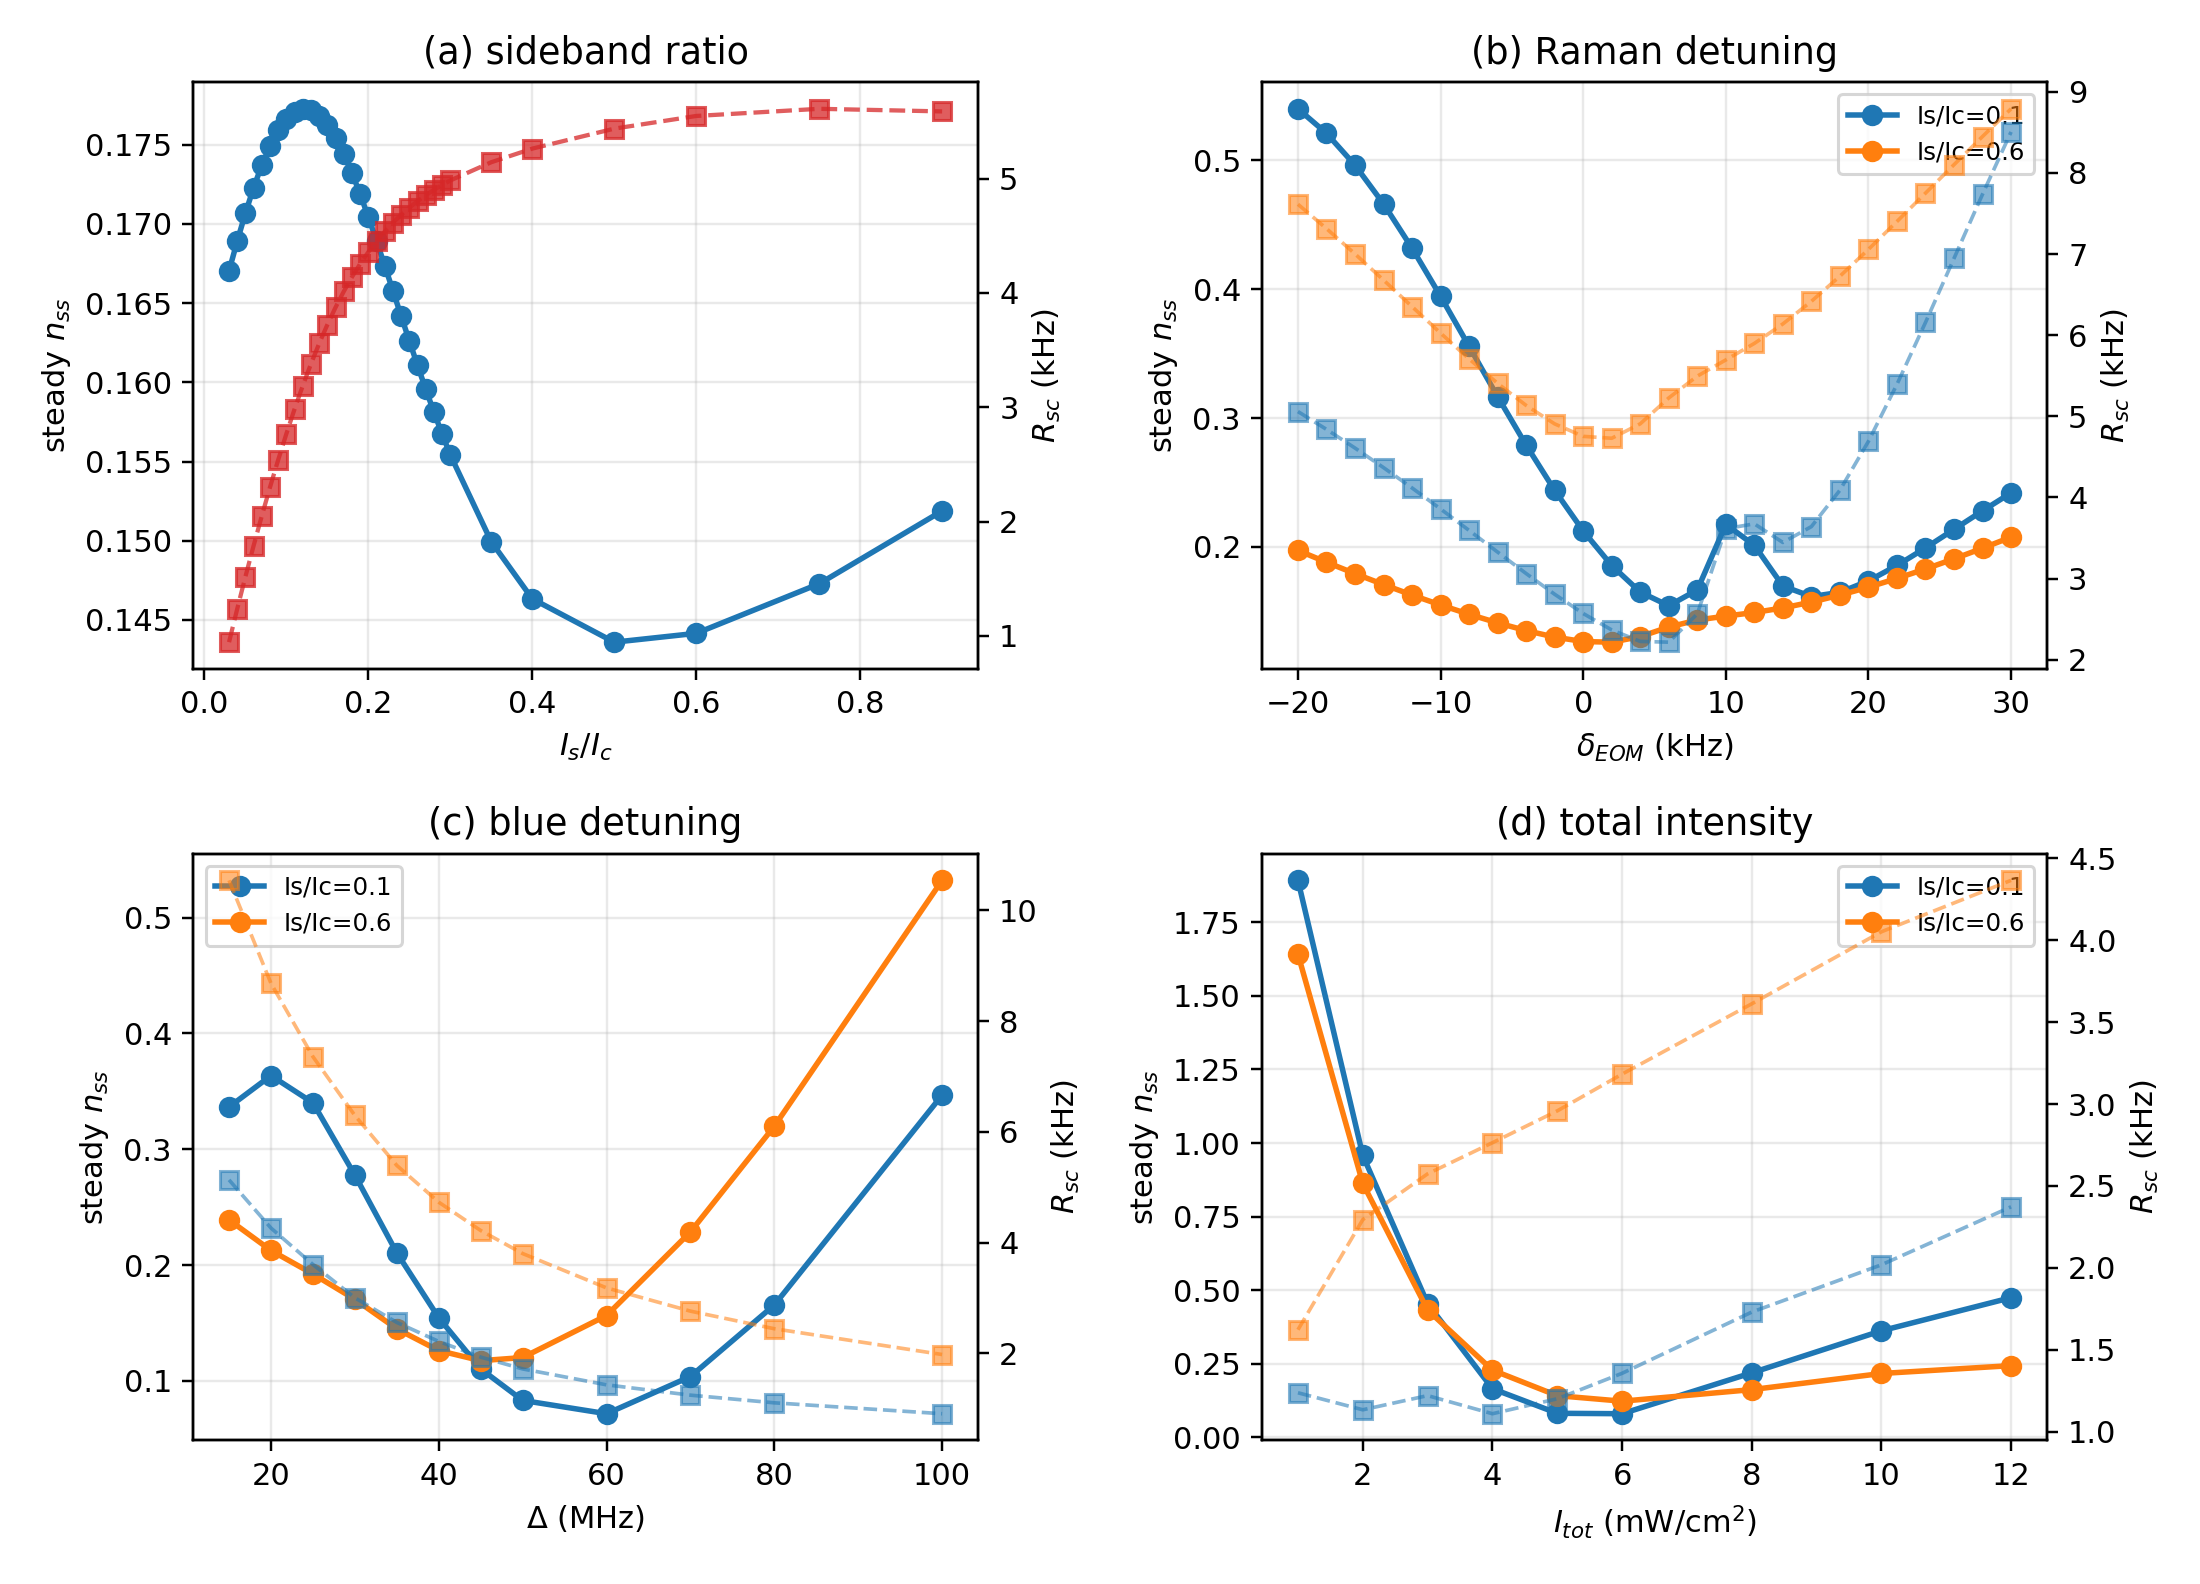
\includegraphics[width=0.96\linewidth]{figures/coarse_scan_overview.png}
  \caption{第一阶段大范围单参数粗扫。实线为稳态平均声子数，虚线为散射率；每次只改变一个参数，其余参数固定在对应扫描的基准点。粗扫用于识别参数趋势和候选区域，不作为最终精确最优解。}
  \label{fig:coarse}
\end{figure}

\begin{table}[H]
  \centering
  \caption{参数搜索流程与每一阶段的用途。}
  \label{tab:search_strategy}
  \begin{tabular}{lll}
    \toprule
    阶段 & 计算设置 & 主要作用 \\
    \midrule
    大范围粗扫 & $n_{\mathrm{Fock}}=6$，单参数扫描 & 判断趋势，定位候选区域 \\
    局部精扫 & $n_{\mathrm{Fock}}=6$，缩小步长 & 比较相邻参数点，确定候选最优点 \\
    高截断复核 & $n_{\mathrm{Fock}}=9$，少量候选点 & 检查高 Fock 态尾部和截断收敛 \\
    时间演化验证 & $n_{\mathrm{Fock}}=6$，$t=5~\mathrm{ms}$ & 计算有限时间冷却曲线和散射代价 \\
    \bottomrule
  \end{tabular}
\end{table}

\subsection{局部精扫与参数依赖}

图 \ref{fig:refine} 展示围绕候选区域的单维精扫。这里的判断不只按稳态平均声子数排序，还同时参考散射率和高 Fock 态尾部。主扫描使用 $n_{\mathrm{Fock}}=6$ 控制计算量，候选点再用 $n_{\mathrm{Fock}}=9$ 检查尾部收敛。

\begin{figure}[H]
  \centering
  \begin{subfigure}{0.48\linewidth}
    \centering
    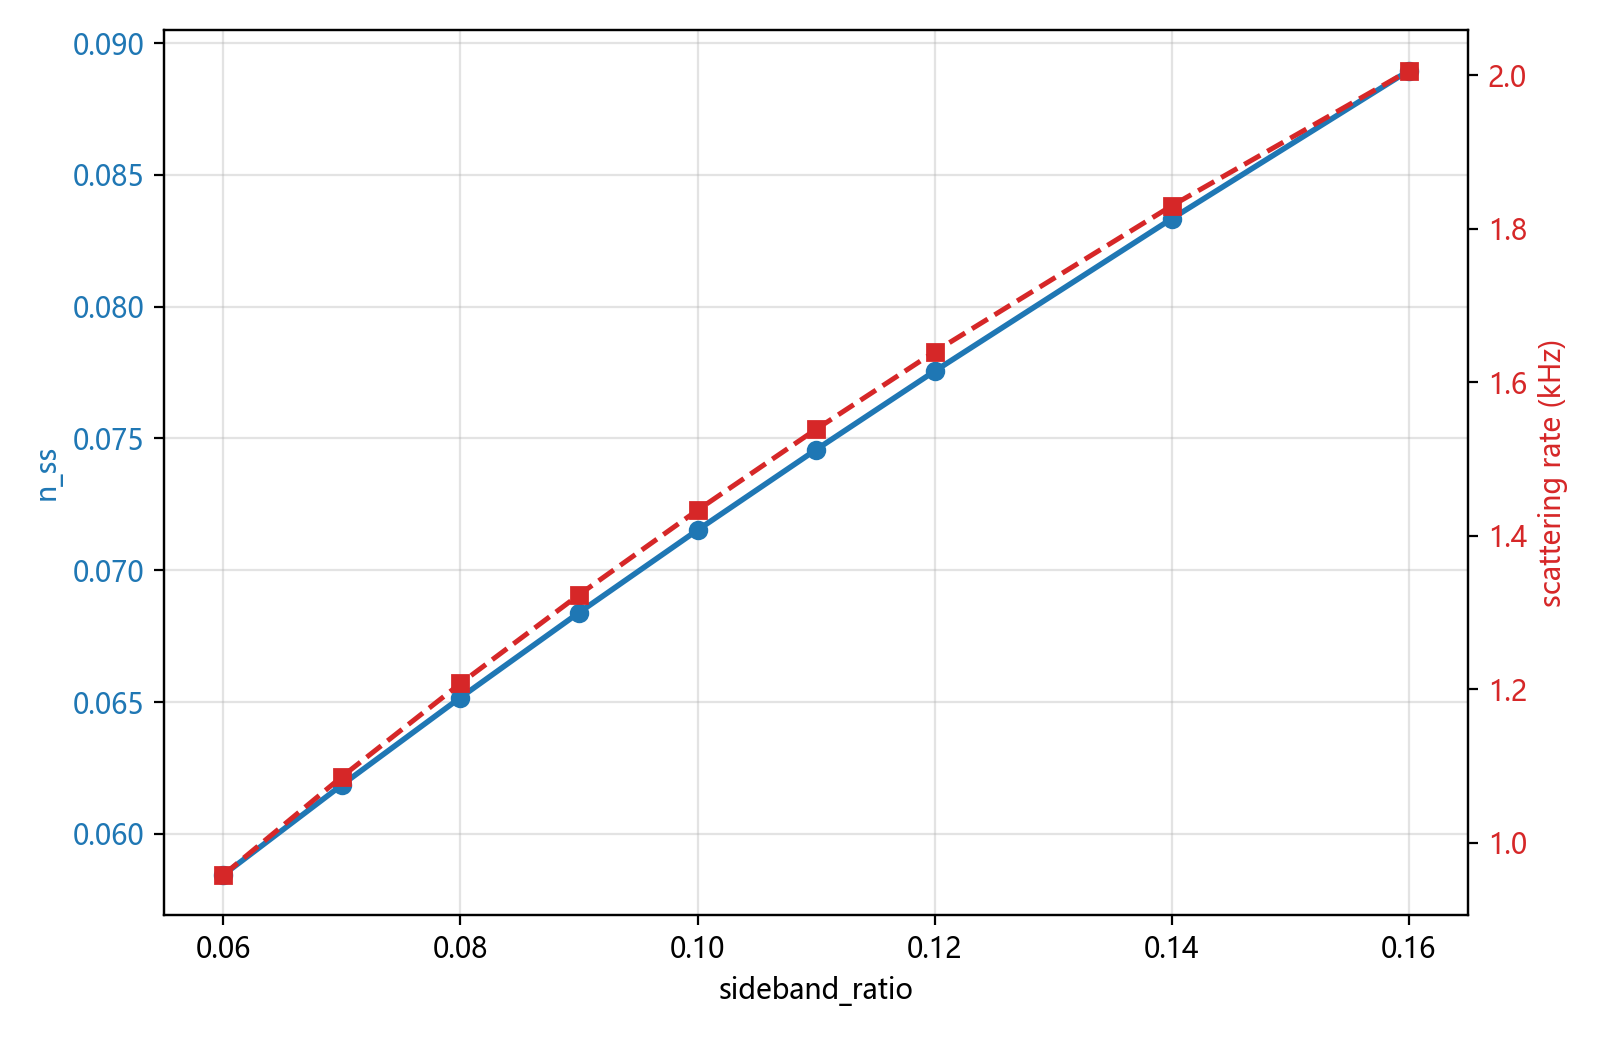
\includegraphics[width=\linewidth]{figures/refine_ratio_initial.png}
    \caption{边带强度比扫描}
  \end{subfigure}
  \begin{subfigure}{0.48\linewidth}
    \centering
    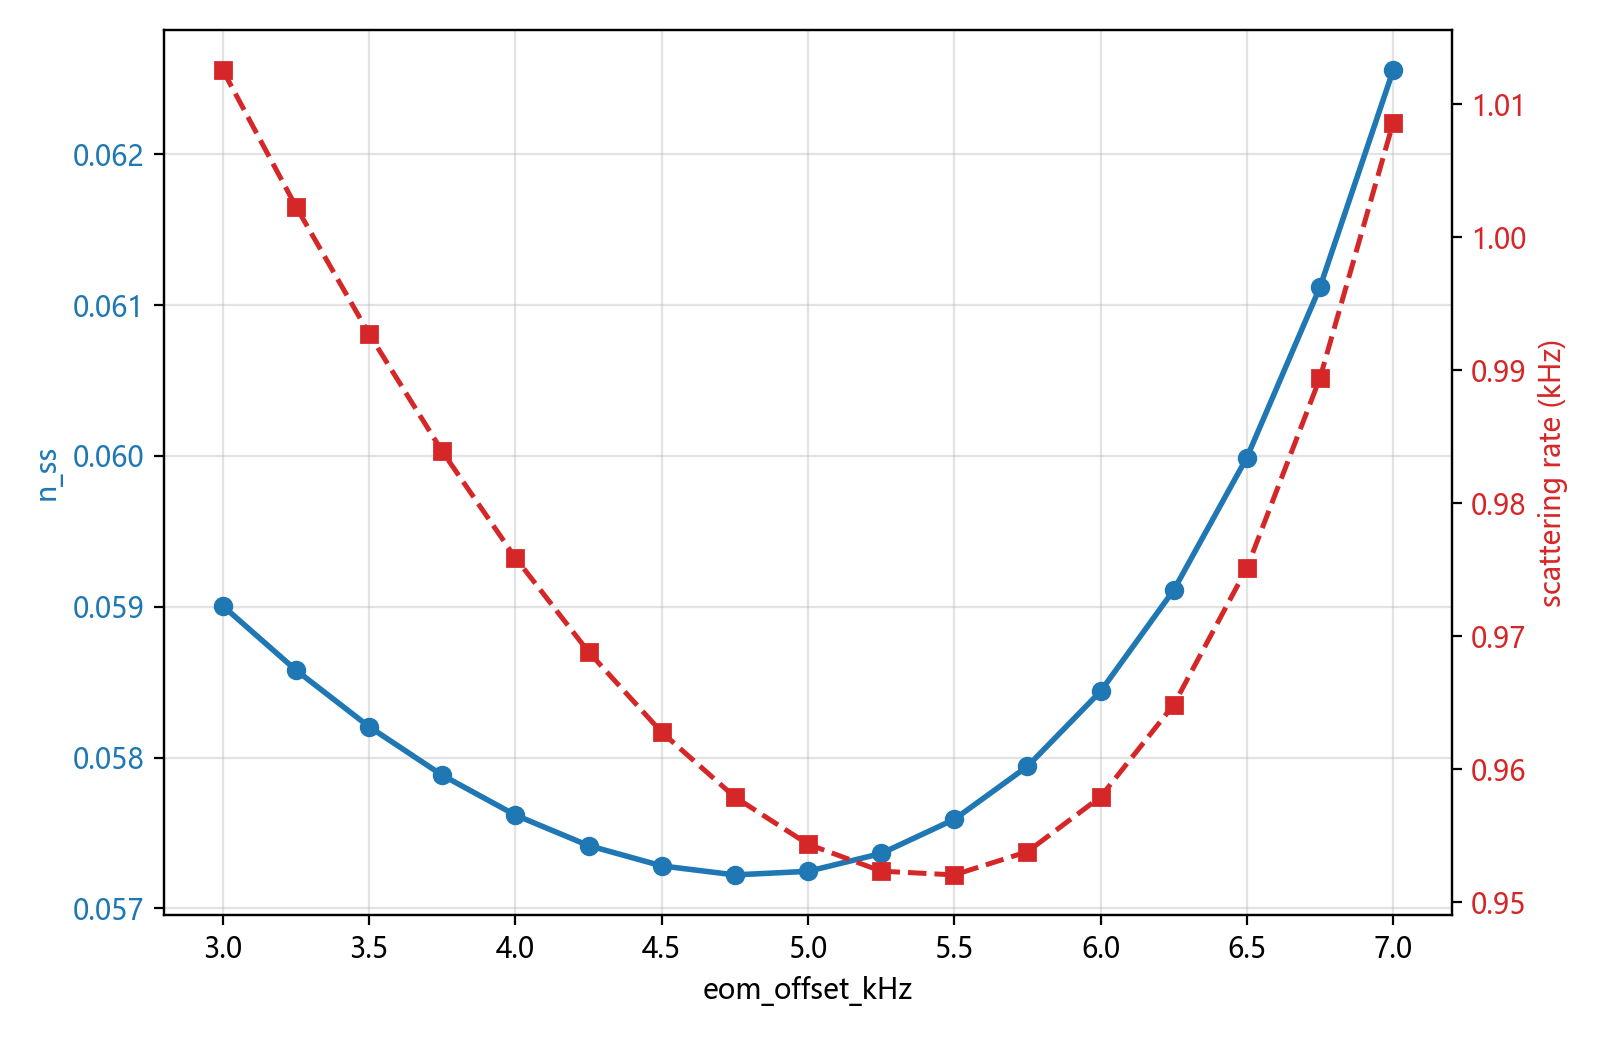
\includegraphics[width=\linewidth]{figures/refine_eom_final.png}
    \caption{双光子失谐扫描}
  \end{subfigure}
  \begin{subfigure}{0.48\linewidth}
    \centering
    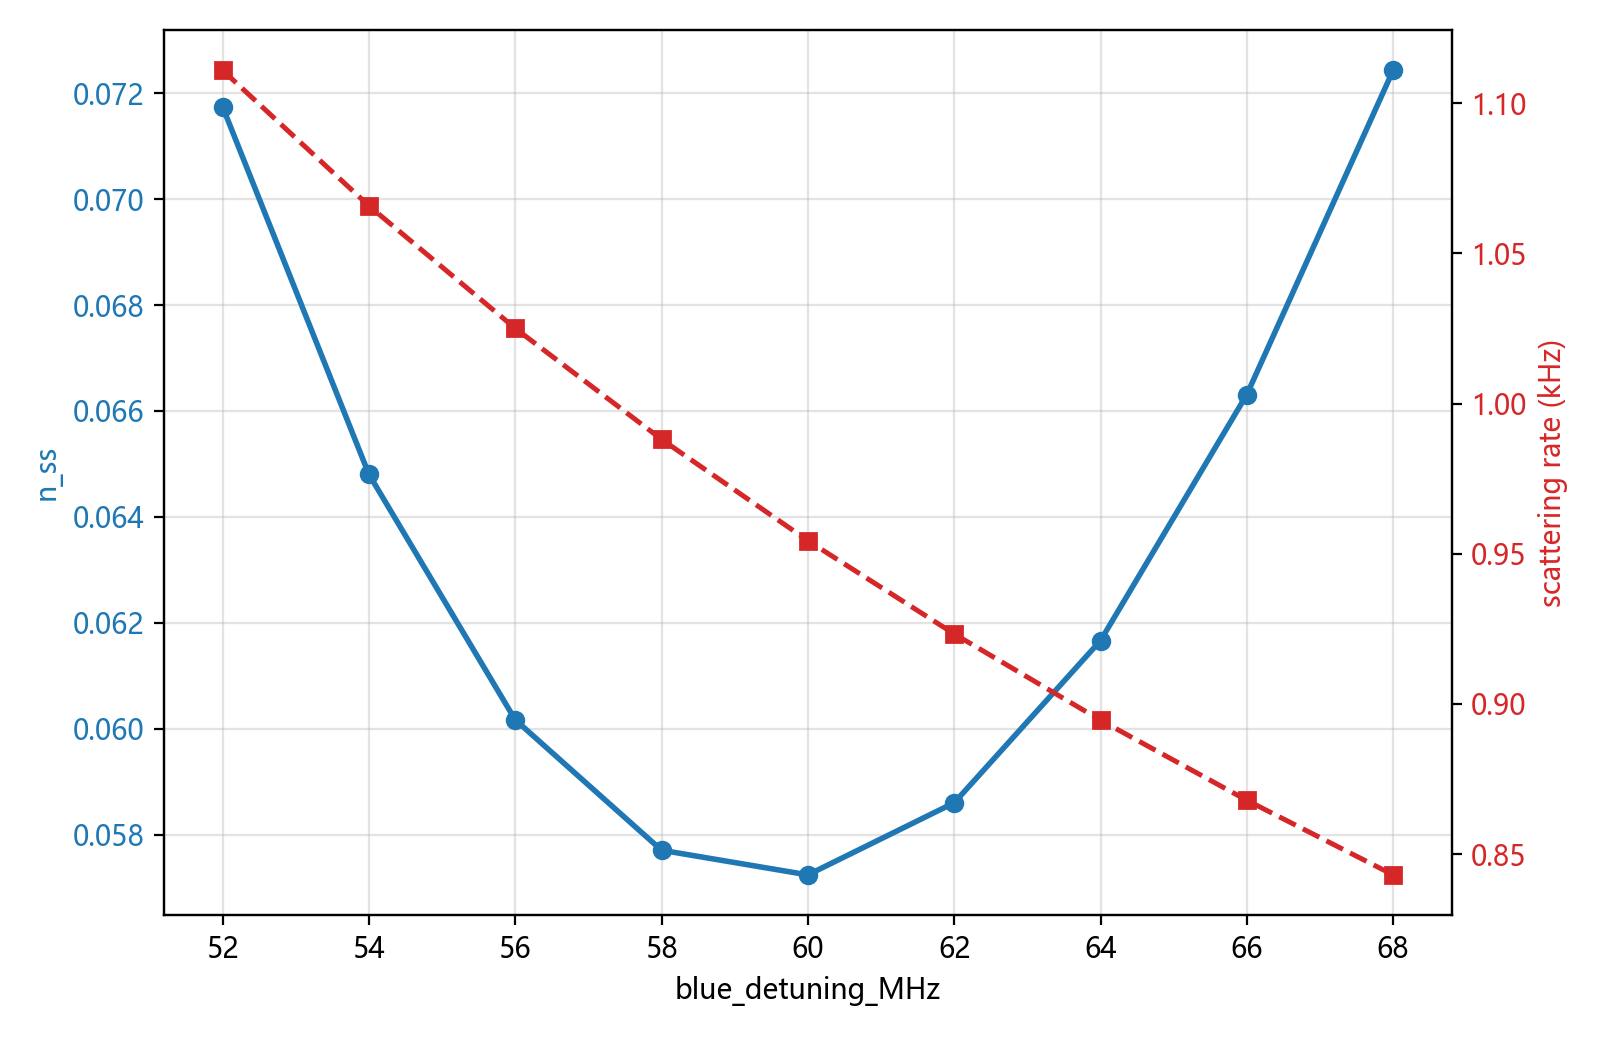
\includegraphics[width=\linewidth]{figures/refine_blue.png}
    \caption{单光子蓝失谐扫描}
  \end{subfigure}
  \begin{subfigure}{0.48\linewidth}
    \centering
    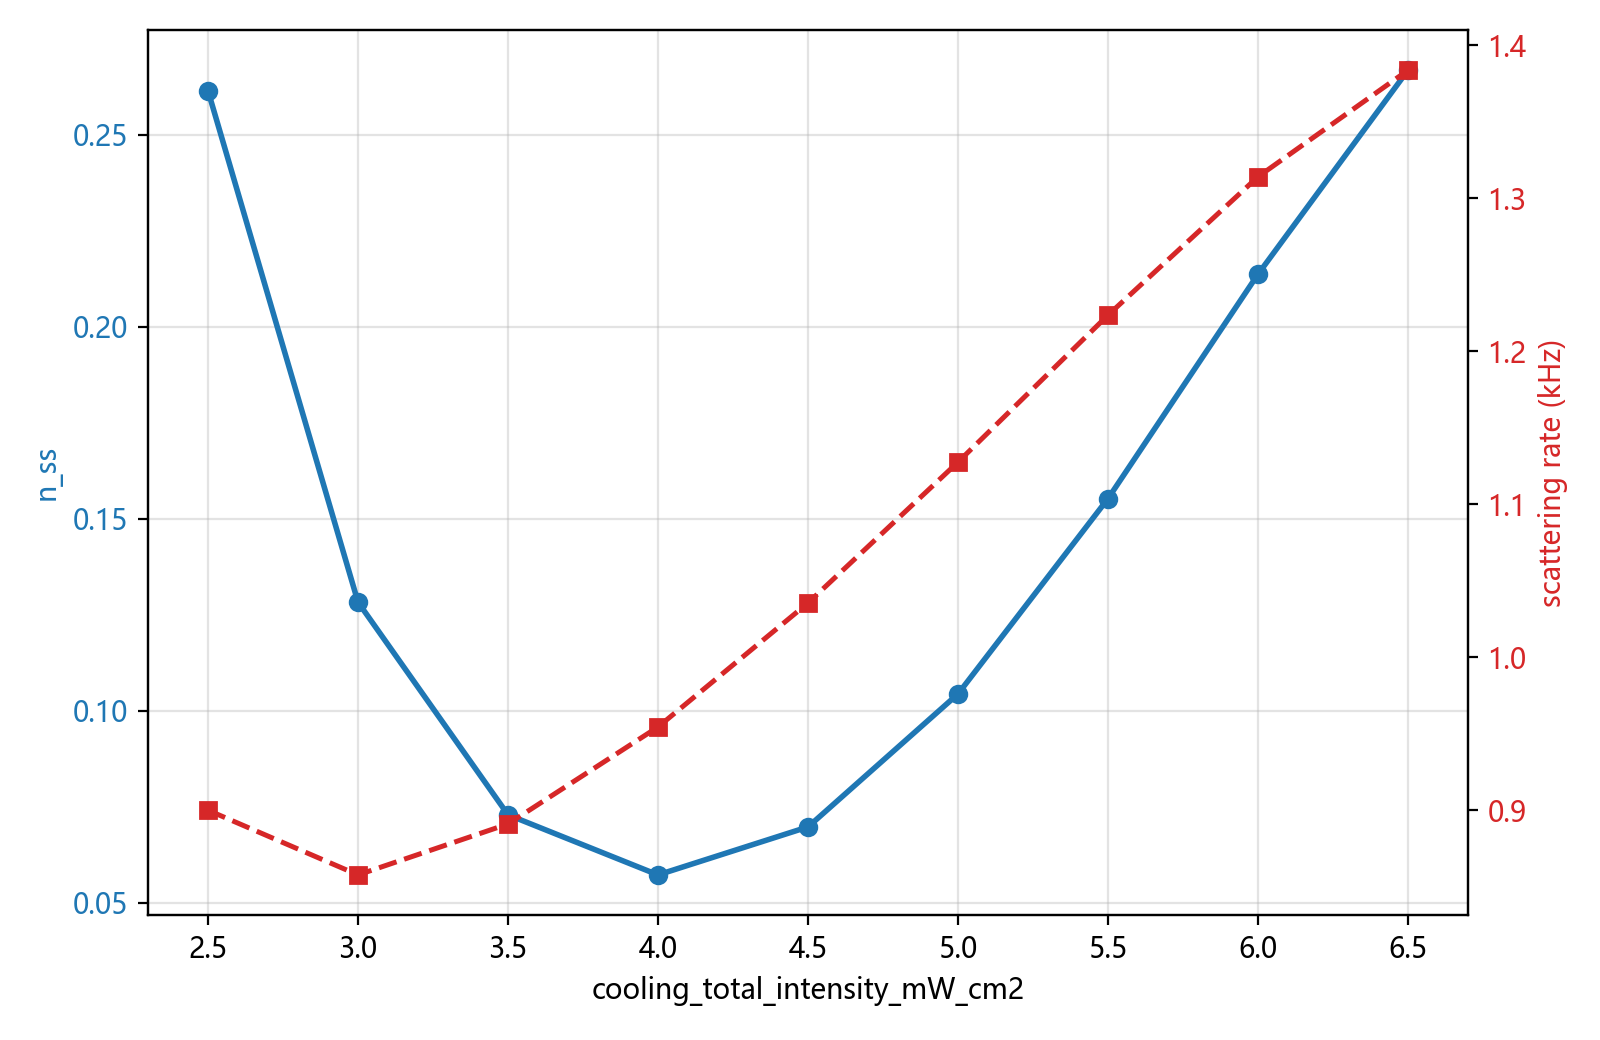
\includegraphics[width=\linewidth]{figures/refine_intensity.png}
    \caption{总光强扫描}
  \end{subfigure}
  \caption{候选区域的局部精扫。蓝色曲线为稳态平均声子数，红色曲线为散射率。每个子图只改变一个参数，其余参数固定在当前候选点。}
  \label{fig:refine}
\end{figure}

低边带比补扫如图 \ref{fig:lowratio} 所示。在当前模型和目标函数下，降低边带比可以同时降低稳态声子数和散射率；但边带比过小也会降低光泵浦速率，使系统在有限时间内更慢接近稳态。因此，稳态最优和有限时间最优需要分开判断。图 \ref{fig:lowratio} 只回答“若等待足够长时间，哪个参数的稳态更冷”；图 \ref{fig:time06} 和图 \ref{fig:comparetime} 则回答“在给定 \(5~\mathrm{ms}\) 冷却窗口内，实际能冷到多少”。

\begin{figure}[H]
  \centering
  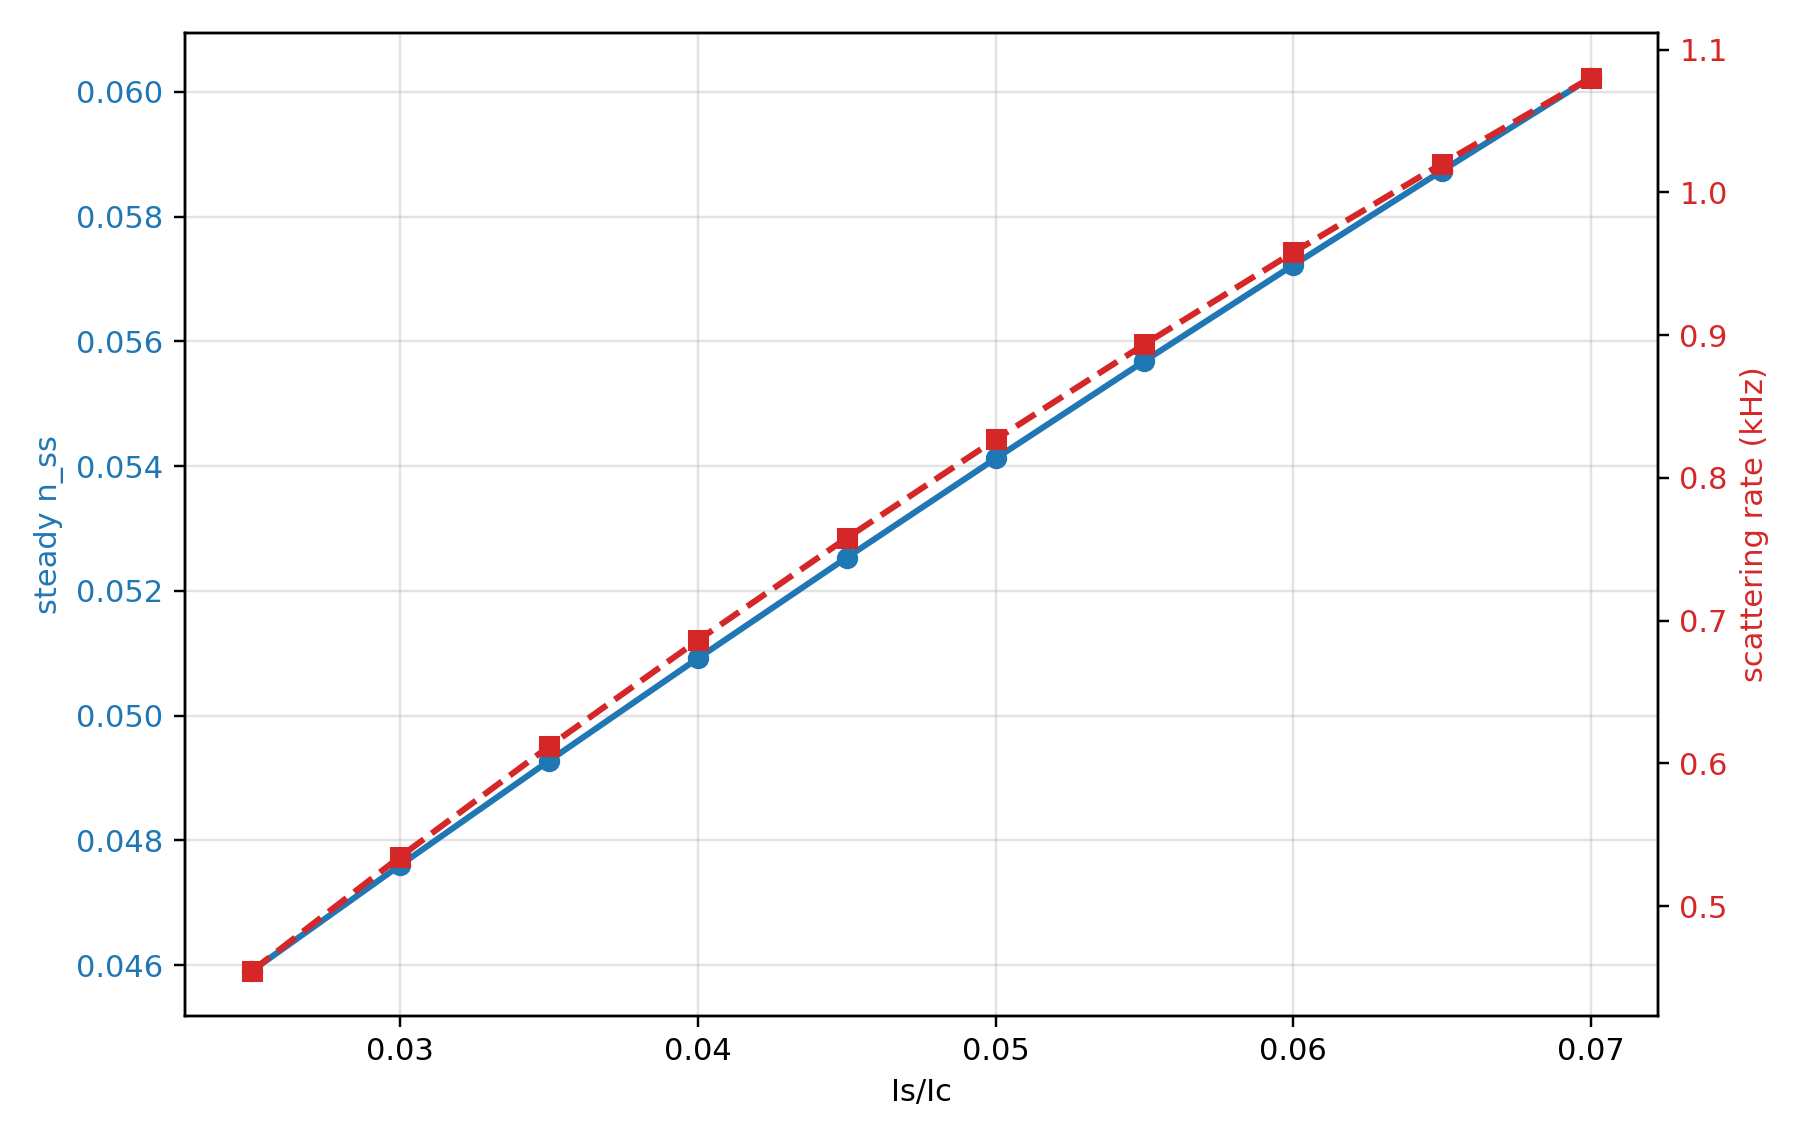
\includegraphics[width=0.78\linewidth]{figures/low_ratio_refine.png}
  \caption{低边带强度比区域的补充扫描。稳态最低和固定 $5~\mathrm{ms}$ 后最低不是同一个优化问题。}
  \label{fig:lowratio}
\end{figure}

\subsection{候选参数点的时间演化验证}

以 $5~\mathrm{ms}$ 后平均声子数最低为目标，候选参数取
\[
I_s/I_c=0.06,\quad
\delta_{\mathrm{EOM}}=4.75~\mathrm{kHz},\quad
\Delta=60~\mathrm{MHz},\quad
I_{\mathrm{tot}}=4~\mathrm{mW/cm^2}.
\]
该点用 $n_{\mathrm{Fock}}=9$ 求稳态，用 $n_{\mathrm{Fock}}=6$ 做完整时间演化。图 \ref{fig:time06} 给出 $n(t)$，红色虚线为高截断稳态参考值。

\begin{figure}[H]
  \centering
  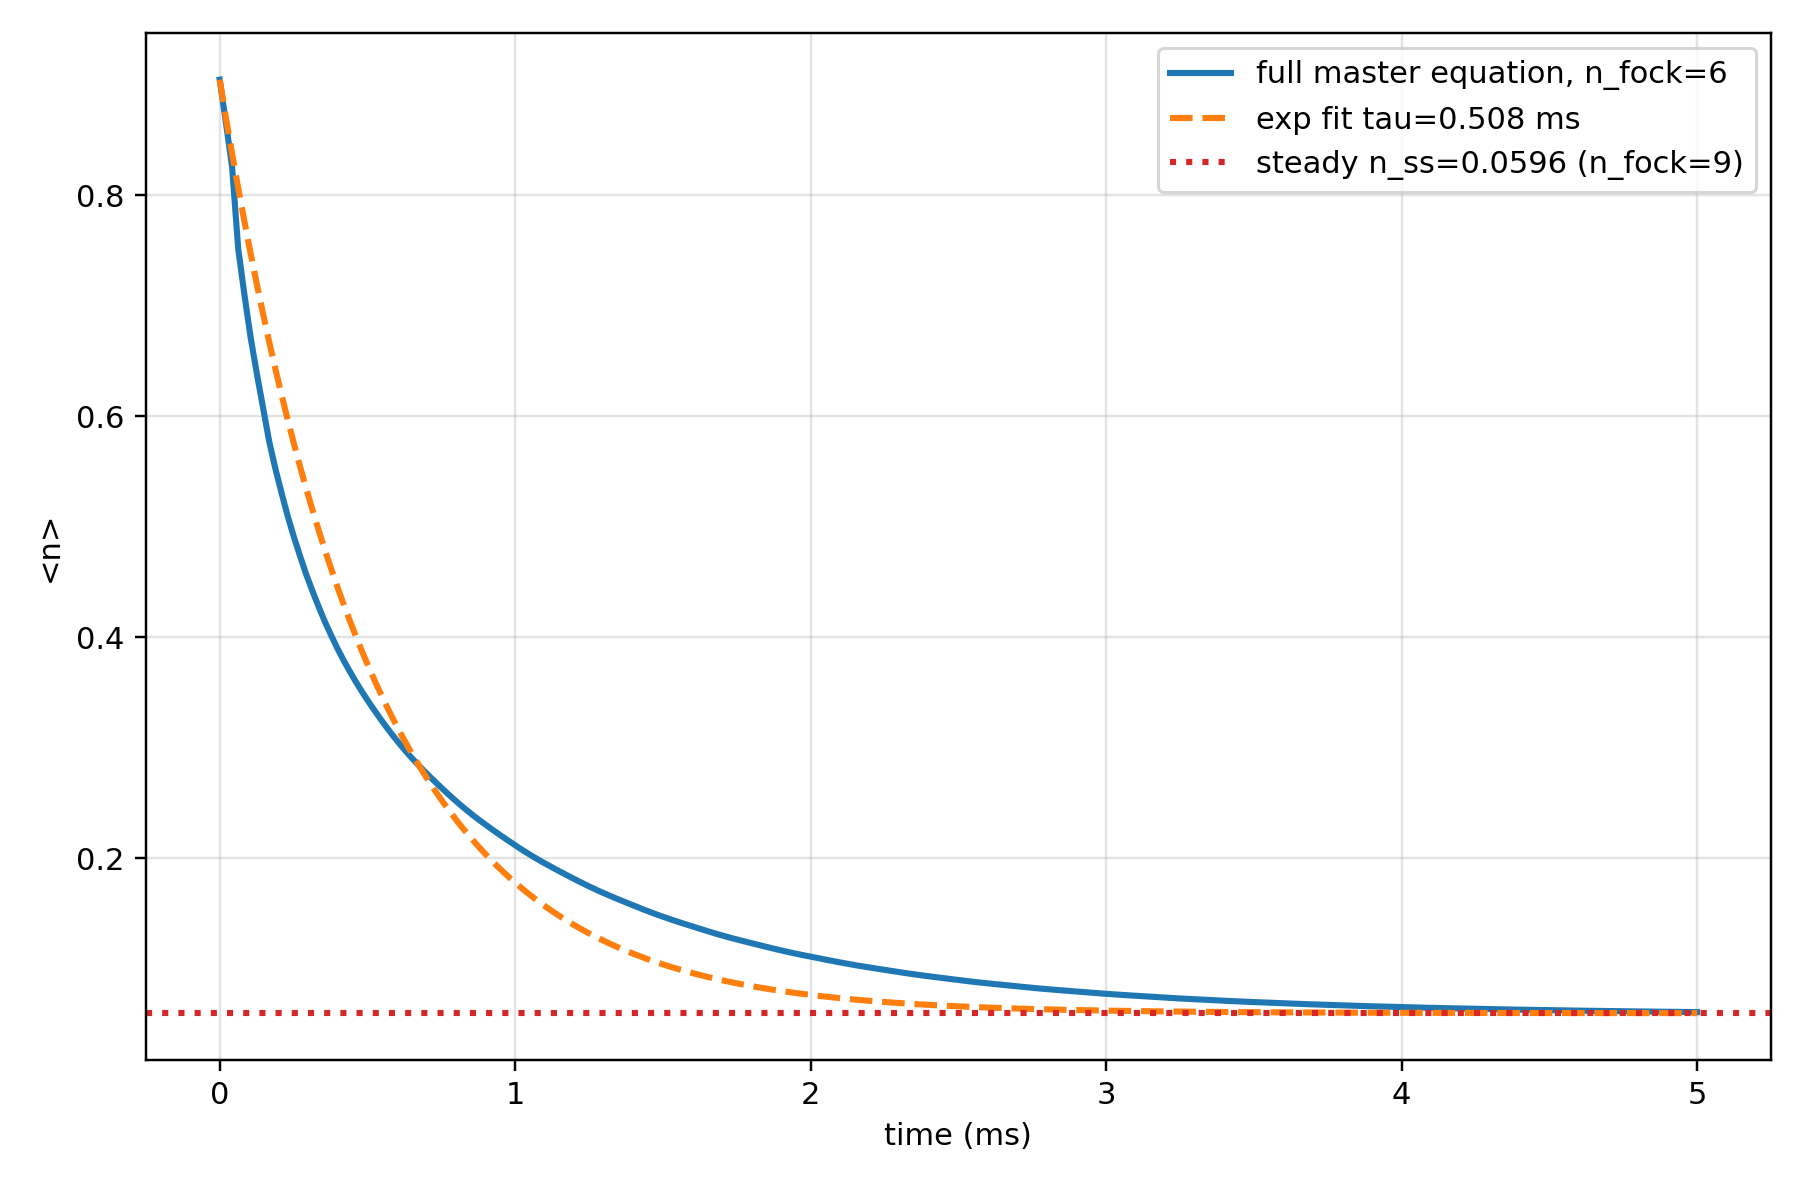
\includegraphics[width=0.82\linewidth]{figures/time_ratio_0p06.png}
  \caption{$I_s/I_c=0.06$ 候选点的完整 Lindblad 时间演化。该点在 $5~\mathrm{ms}$ 内已经基本接近稳态。}
  \label{fig:time06}
\end{figure}

为了说明有限时间判据的重要性，图 \ref{fig:comparetime} 对比了 $I_s/I_c=0.06$ 与低散射参考点 $I_s/I_c=0.025$。后者的稳态声子数和散射率更低，但冷却更慢，因此在 $5~\mathrm{ms}$ 这个固定时间上反而给出略高的声子数。也就是说，\(I_s/I_c=0.025\) 更适合作为低散射、低稳态温度的参考方案；若只看有限冷却窗口内的最低声子数，\(I_s/I_c=0.06\) 更合适。

\begin{figure}[H]
  \centering
  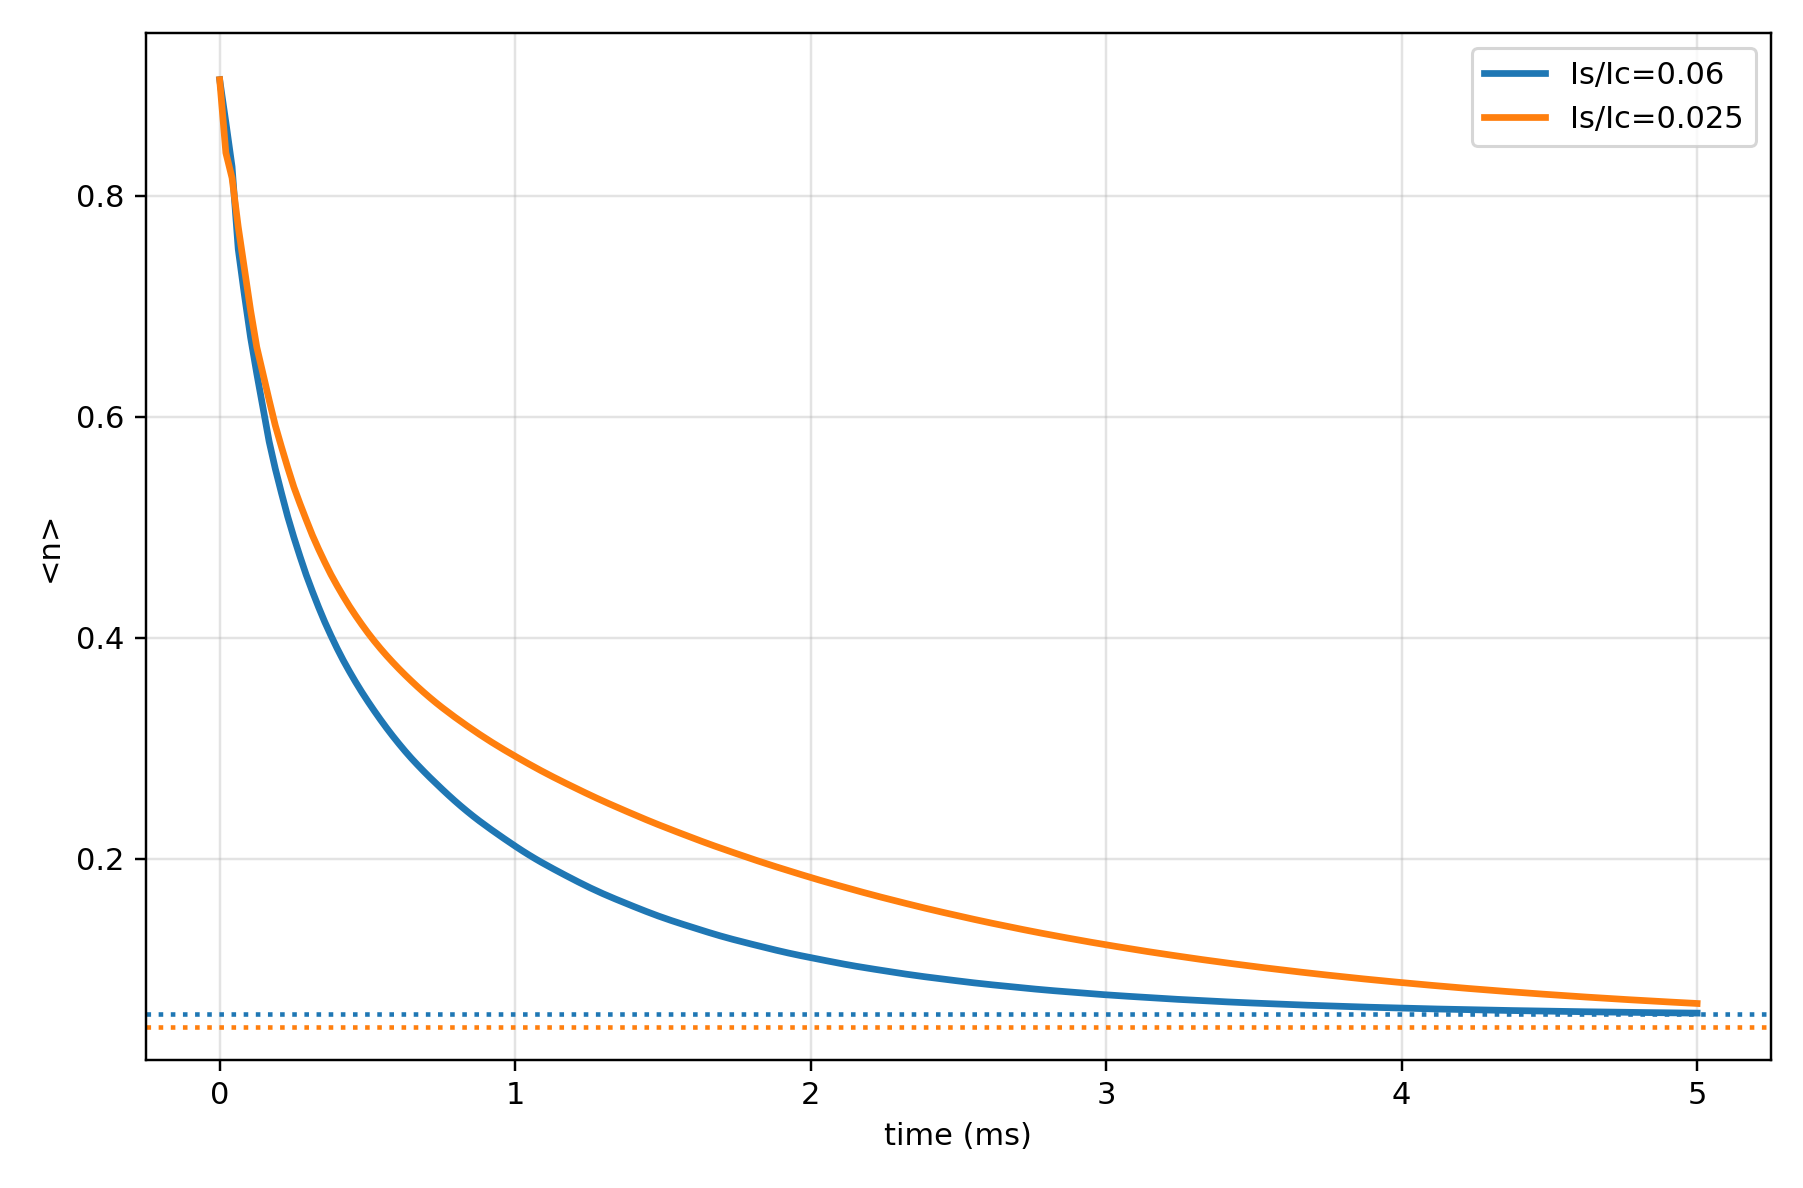
\includegraphics[width=0.82\linewidth]{figures/time_curve_comparison.png}
  \caption{两个边带强度比的完整时间演化对比。点线为各自的高截断稳态值。}
  \label{fig:comparetime}
\end{figure}

\begin{table}[H]
  \centering
  \caption{有限时间冷却判据下的代表性参数点比较。表中两行分别对应“最低 \(5~\mathrm{ms}\) 后声子数”和“低散射、低稳态声子数”两种优化目标。}
  \label{tab:cooling_summary}
  \begin{tabular}{lccccc p{3.4cm}}
    \toprule
    优化目标 & $I_s/I_c$ & $n_{\mathrm{ss}}$ & $n(5~\mathrm{ms})$ & $\tau$ (ms) & $R_{\mathrm{sc}}$ (kHz) & 结论 \\
    \midrule
    有限时间最低声子数 & 0.060 & 0.0596 & 0.0606 & 0.508 & 0.960 & \(5~\mathrm{ms}\) 内已接近稳态，是最终采用的冷却参数 \\
    低散射/低稳态参考 & 0.025 & 0.0479 & 0.0693 & 0.817 & 0.455 & 稳态和散射率更优，但在 \(5~\mathrm{ms}\) 内冷却不足 \\
    \bottomrule
  \end{tabular}
\end{table}

图 \ref{fig:pe} 给出最优冷却点的激发态布居。为避免光场刚打开时的快速瞬态掩盖准稳态散射行为，图中从 \(t=0.02~\mathrm{ms}\) 开始绘制，并采用对数纵轴。冷却进入准稳态后，激发态布居降至 \(10^{-5}\) 量级，对应 kHz 量级散射率。这与 grey molasses 的设计目标一致：保留足够的光泵浦完成冷却，同时尽量让冷原子停留在低散射暗态附近。

\begin{figure}[H]
  \centering
  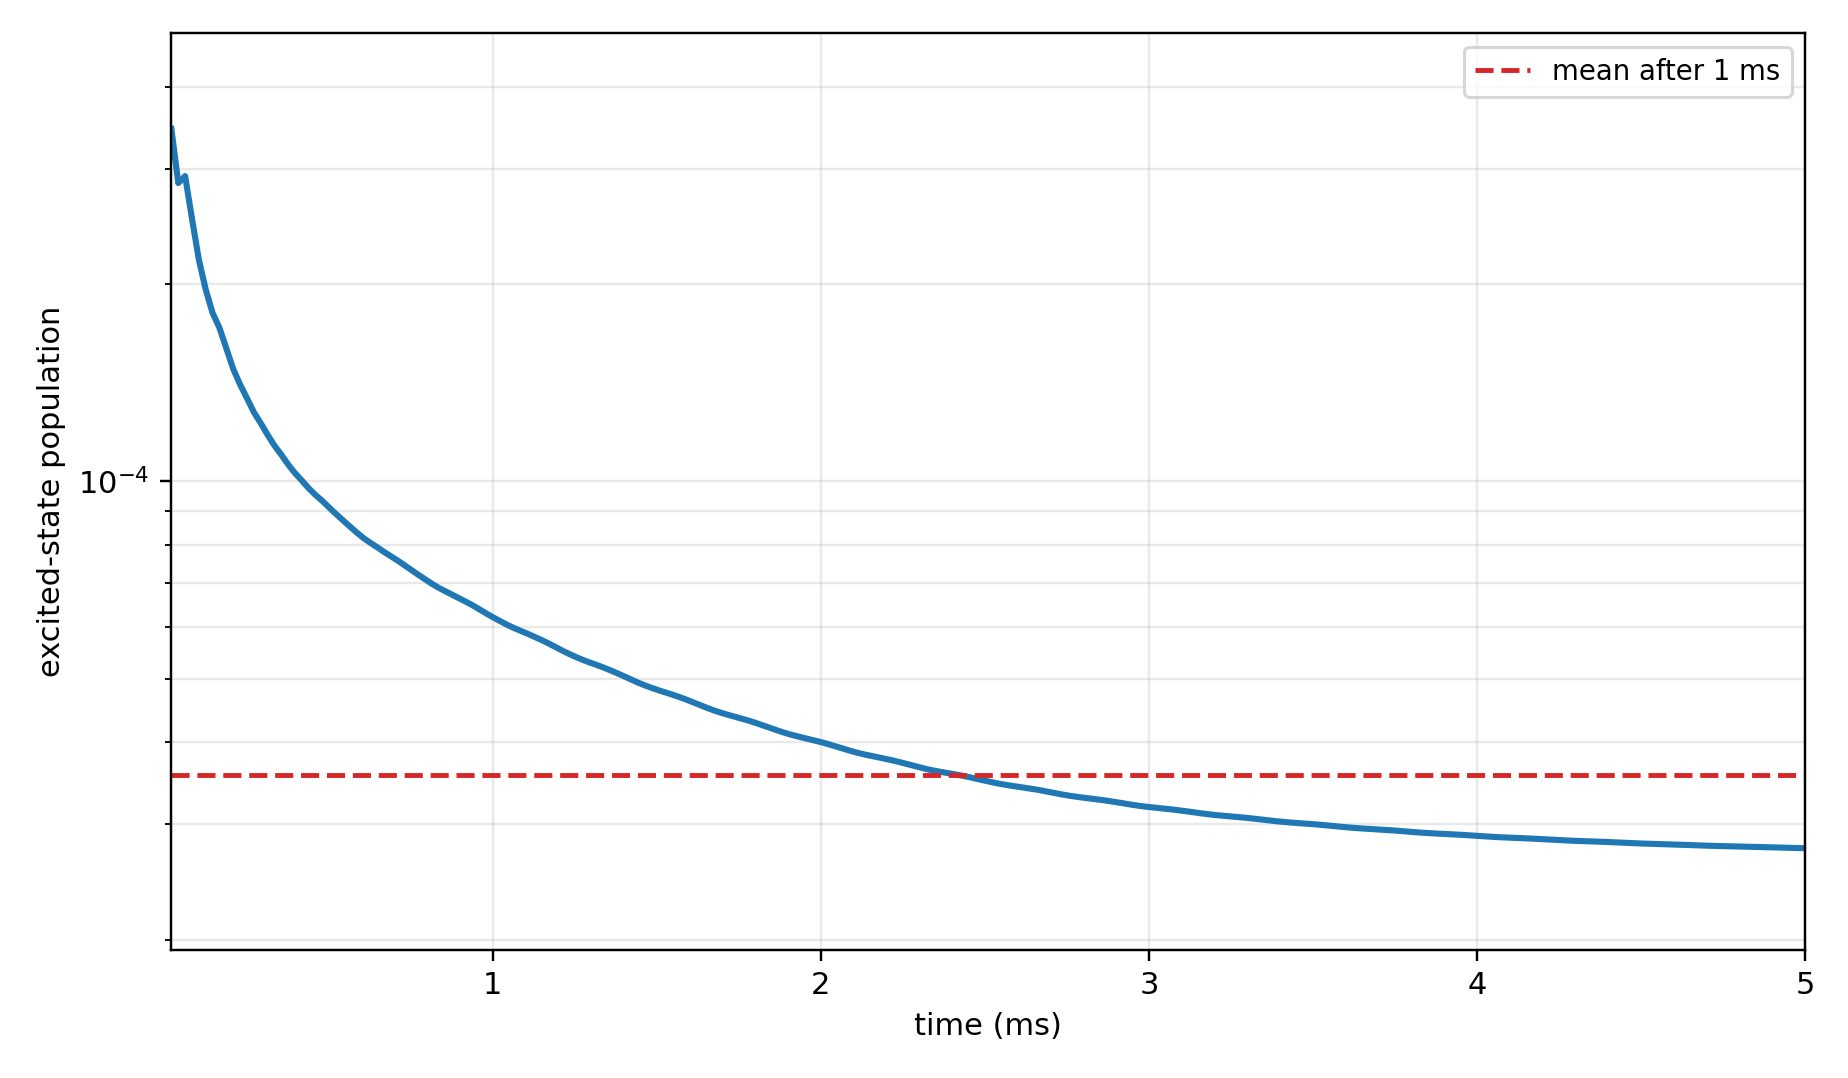
\includegraphics[width=0.80\linewidth]{figures/pe_ratio_0p06_quasisteady.png}
  \caption{$I_s/I_c=0.06$ 候选点的激发态布居随时间变化。图中排除了最初 \(0.02~\mathrm{ms}\) 的光学瞬态，以突出与散射率相关的准稳态布居。}
  \label{fig:pe}
\end{figure}

\section{装载率模拟结果}

\subsection{蓝失谐对碰撞阻塞装载的影响}

装载率扫描沿用前面得到的冷却参数中的光强、边带比和双光子失谐：
\[
I_s/I_c=0.06,\qquad
\delta_{\mathrm{EOM}}=4.75~\mathrm{kHz},\qquad
I_{\mathrm{tot}}=4~\mathrm{mW/cm^2}.
\]
在此基础上扫描蓝失谐 $\Delta=20$--$65~\mathrm{MHz}$。每个点先用 $n_{\mathrm{Fock}}=6$ 求冷却稳态，得到冷原子温度和散射率；再将这些量送入碰撞阻塞模块，计算 $\beta_1,\beta_2$；最后积分式 \eqref{eq:loading_rate} 到 $2~\mathrm{s}$。

\begin{figure}[H]
  \centering
  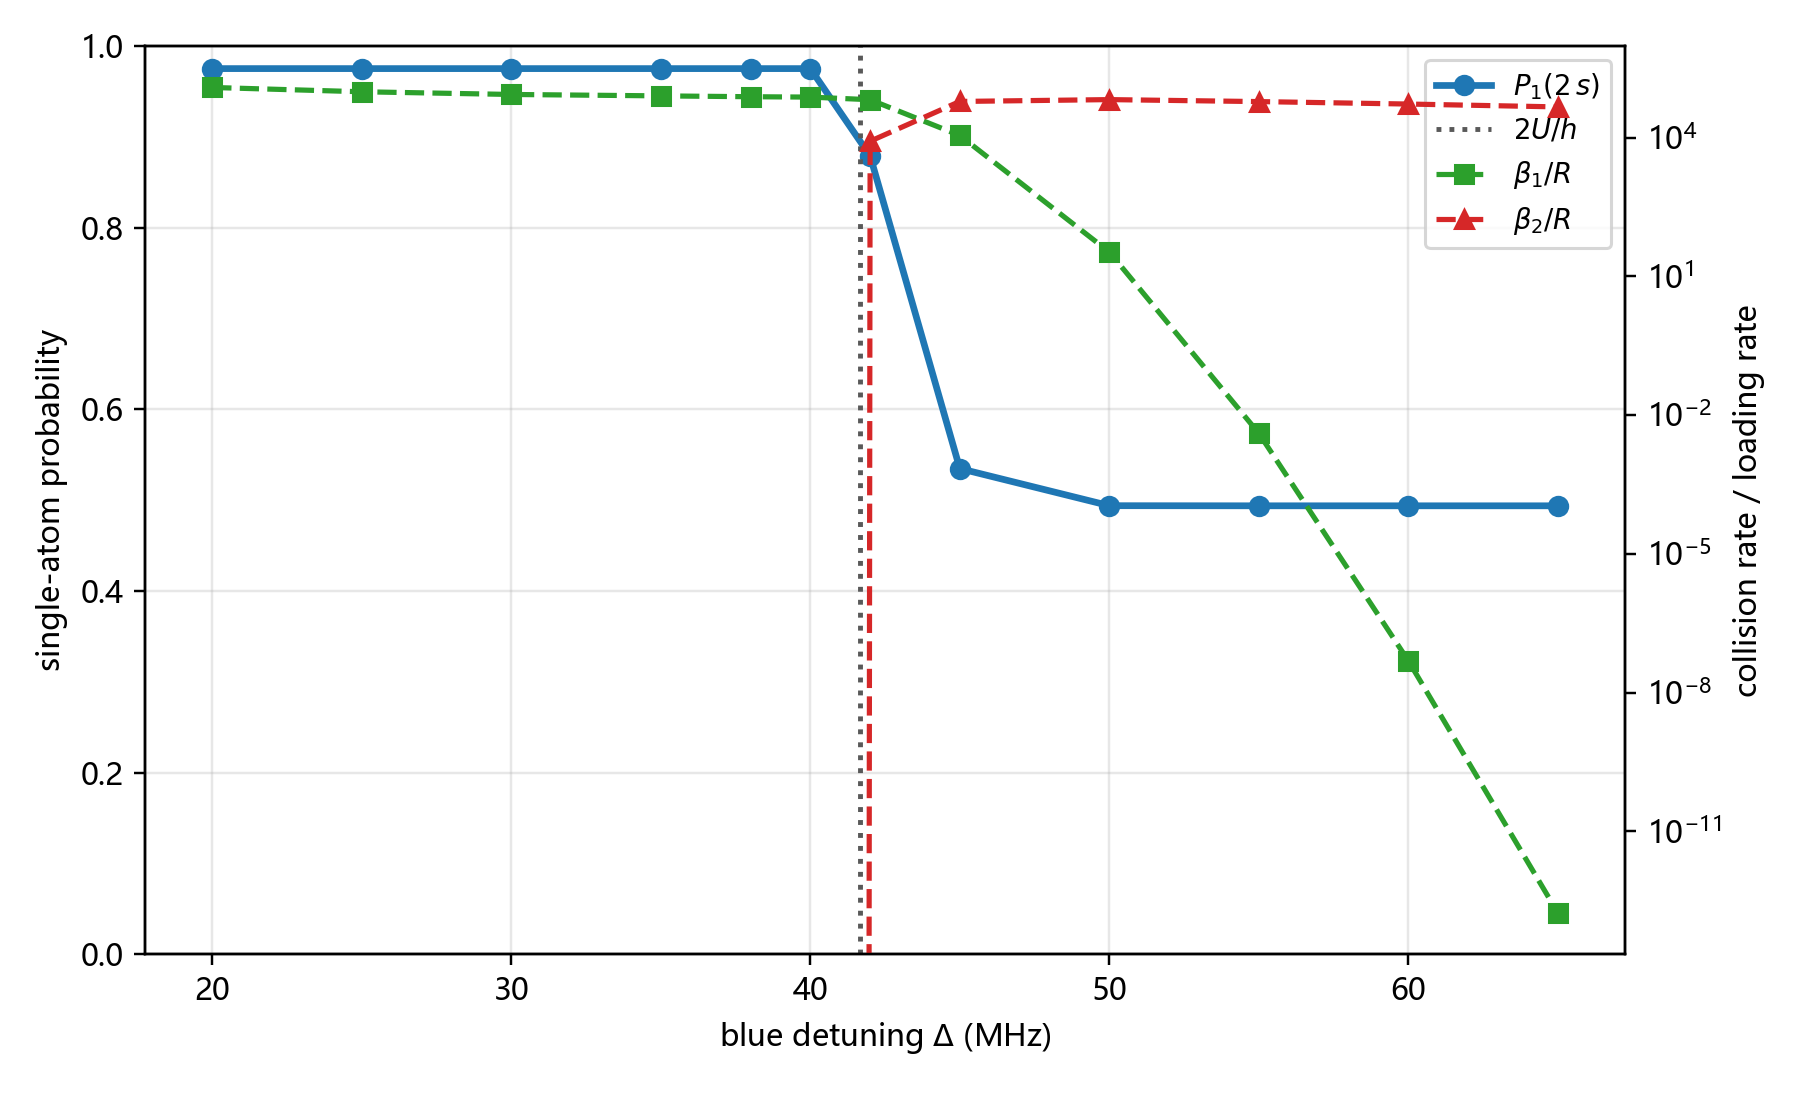
\includegraphics[width=0.84\linewidth]{figures/loading_detuning_scan.png}
  \caption{蓝失谐对单原子装载概率的影响。灰色虚线为 $2U/h=41.7~\mathrm{MHz}$ 阈值；绿色和红色曲线分别为单原子损失通道和双原子损失通道相对 MOT 装载率 $R$ 的大小。}
  \label{fig:loading_scan}
\end{figure}

图 \ref{fig:loading_scan} 给出蓝失谐对装载率的影响。低于 $2U/h$ 时，$\beta_1/R$ 很大而 $\beta_2/R\simeq0$，二体事件主要转化为单原子保留，因此 $P_1(2~\mathrm{s})$ 接近由 $R$ 和背景寿命决定的上限，约为 $0.975$。当 $\Delta$ 越过 $2U/h$ 后，$\beta_2$ 迅速变大，双原子共同逃逸通道打开，$P_1$ 从 $0.879$ 进一步降到约 $0.49$。这一结果说明，蓝失谐不仅影响冷却效率，也会通过碰撞能量阈值直接改变装载结果。

\begin{table}[H]
  \centering
  \caption{装载率扫描中的代表点。默认阱深 $U=1~\mathrm{mK}$，因此阈值 $2U/h=41.7~\mathrm{MHz}$。}
  \label{tab:loading_summary}
  \begin{tabular}{cccccc}
    \toprule
    $\Delta$ (MHz) & $n_{\mathrm{ss}}$ & $\beta_1/R$ & $\beta_2/R$ & $P_1(2~\mathrm{s})$ & 物理区间 \\
    \midrule
    20 & 0.396 & $1.22\times10^5$ & 0 & 0.975 & 单原子保留平台 \\
    35 & 0.234 & $8.01\times10^4$ & 0 & 0.975 & 单原子保留平台 \\
    40 & 0.171 & $7.54\times10^4$ & 0 & 0.975 & 接近阈值下方 \\
    42 & 0.148 & $6.62\times10^4$ & $8.37\times10^3$ & 0.879 & 阈值交叉 \\
    45 & 0.118 & $1.11\times10^4$ & $6.07\times10^4$ & 0.535 & 双原子逃逸增强 \\
    60 & 0.057 & $4.88\times10^{-8}$ & $5.34\times10^4$ & 0.494 & 冷却强但装载差 \\
    \bottomrule
  \end{tabular}
\end{table}

\subsection{单原子装载概率的时间演化}

图 \ref{fig:loading_curves} 给出几个蓝失谐点的 $P_1(t)$。在 $20$ 和 $35~\mathrm{MHz}$，曲线在约一秒内接近饱和；在 $45$ 和 $60~\mathrm{MHz}$，由于双原子损失通道较强，最终只能停在约 $0.5$ 附近。

\begin{figure}[H]
  \centering
  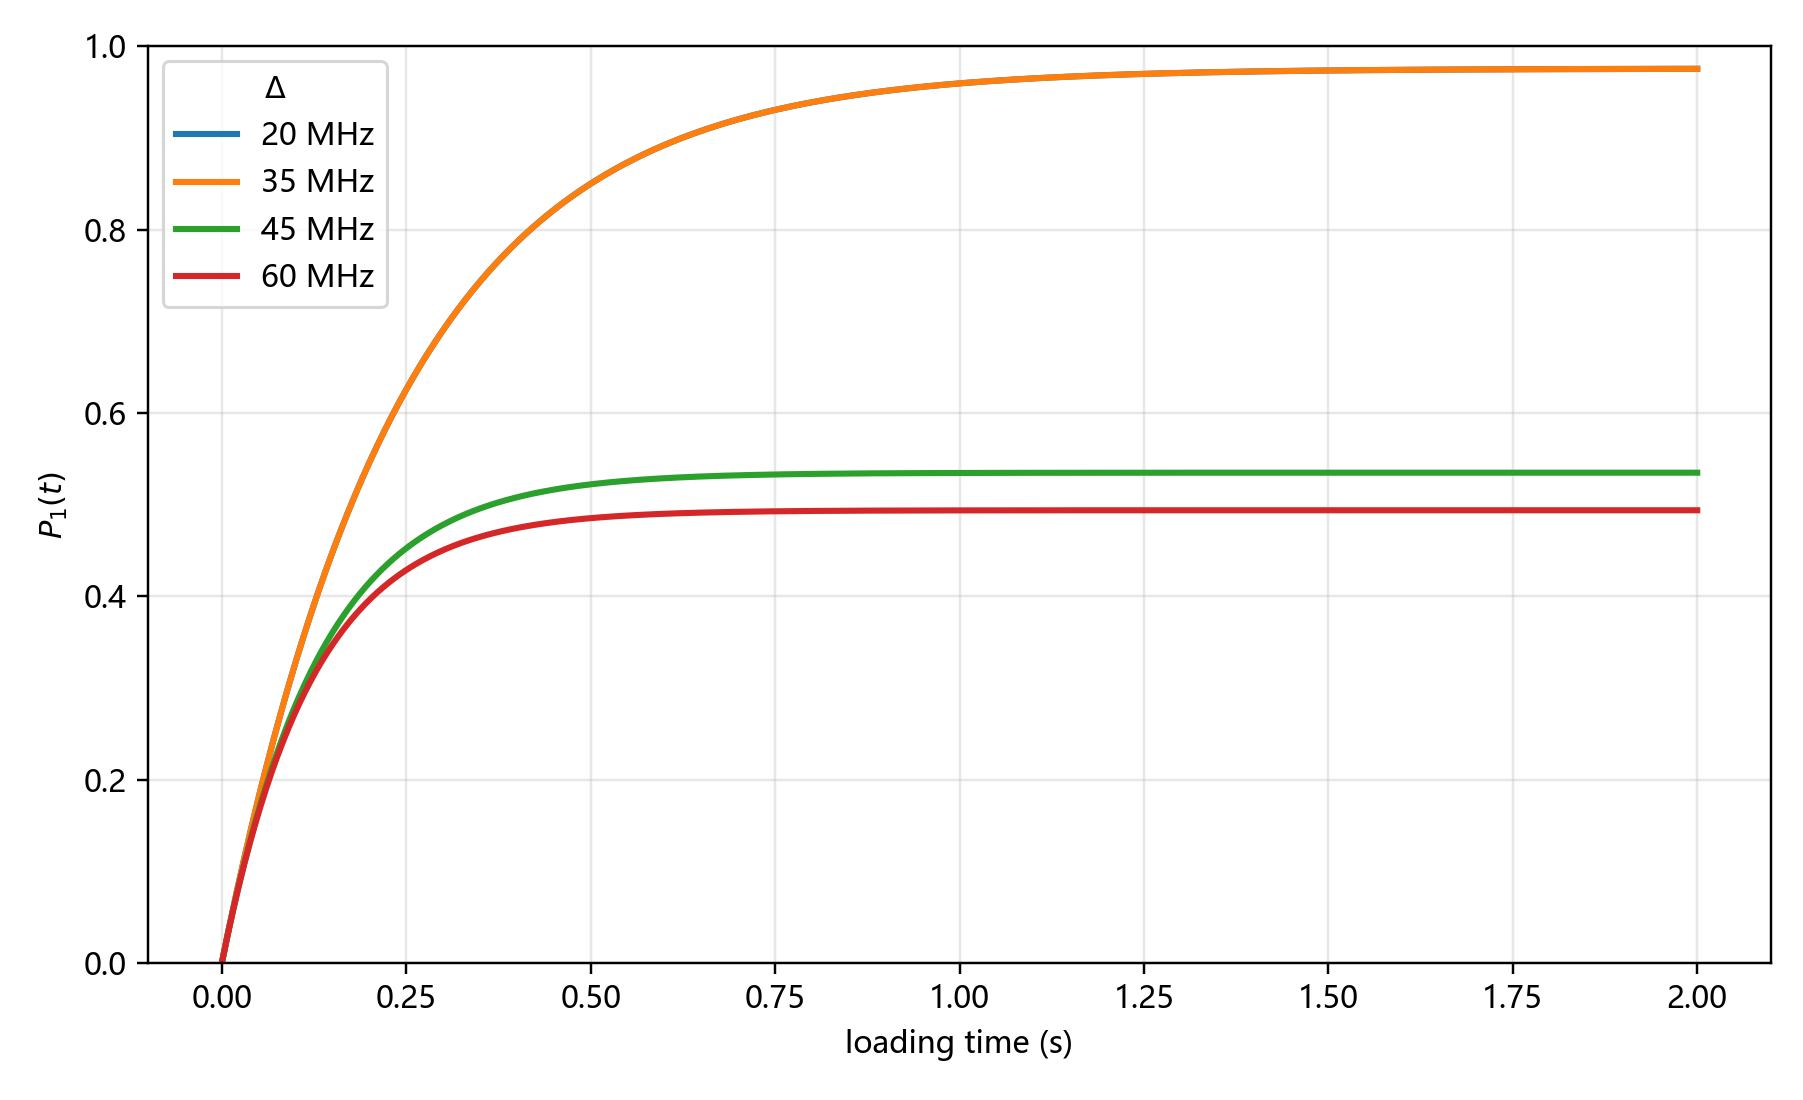
\includegraphics[width=0.84\linewidth]{figures/loading_time_curves.png}
  \caption{不同蓝失谐下的单原子概率 $P_1(t)$。}
  \label{fig:loading_curves}
\end{figure}

图 \ref{fig:loading_best} 展示装载率最优平台上一个代表点的 $P_0,P_1,P_2$。双原子概率始终很小，因为一旦装入第二个原子，强二体碰撞会快速把系统带回单原子状态。

\begin{figure}[H]
  \centering
  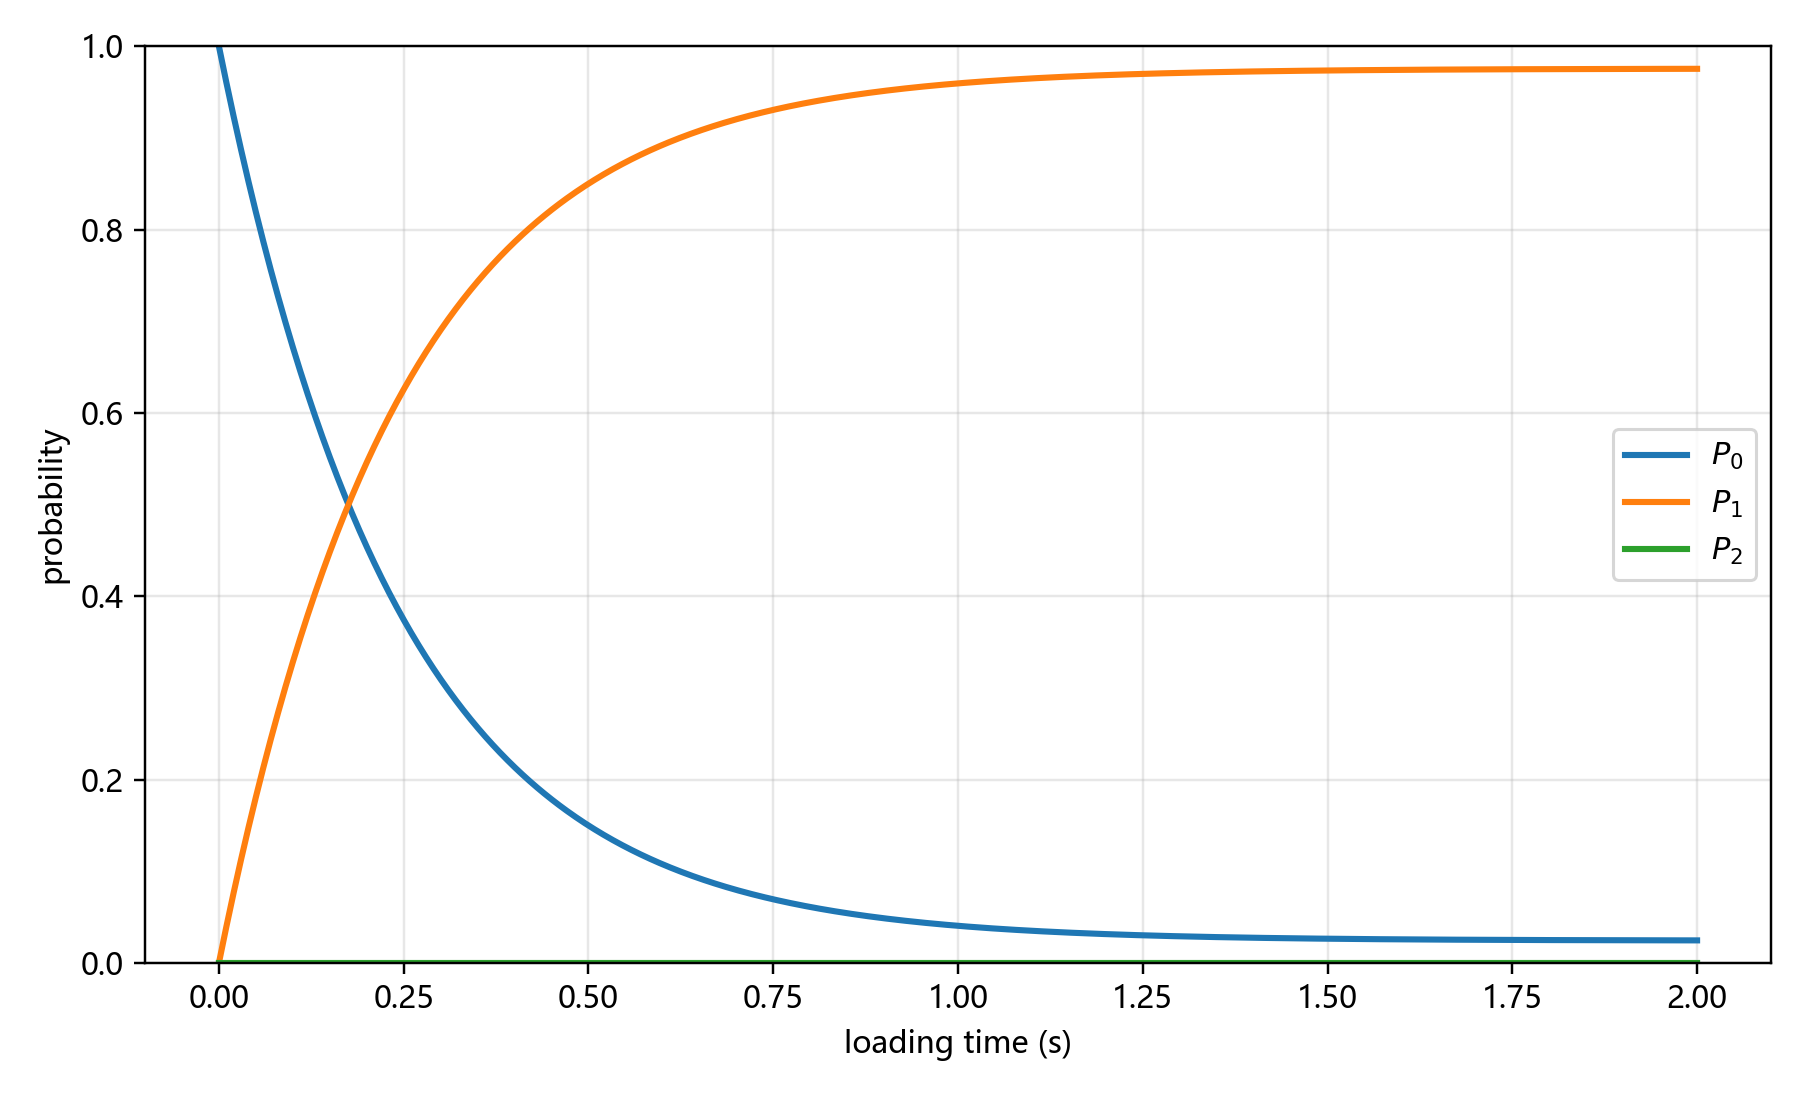
\includegraphics[width=0.84\linewidth]{figures/loading_best_state_probabilities.png}
  \caption{装载率最优平台代表点的 $P_0,P_1,P_2$ 时间演化。}
  \label{fig:loading_best}
\end{figure}

\subsection{冷却指标与装载指标的参数权衡}

把冷却指标和装载指标放在一起看，可以得到以下参数权衡：
\begin{itemize}
  \item 若目标是最终冷却，$\Delta=60~\mathrm{MHz}$ 给出较低的 $n_{\mathrm{ss}}$ 和 $n(5~\mathrm{ms})$；
  \item 若目标是单原子装载率，$\Delta<2U/h$ 的低蓝失谐平台更有利于单原子保留；
  \item 若要求同一组光参数兼顾装载率和冷却温度，$\Delta\simeq38$--$40~\mathrm{MHz}$ 比 $60~\mathrm{MHz}$ 更适合作为折中区域：该区间仍保持高装载率，同时冷却稳态声子数低于 $20$--$30~\mathrm{MHz}$ 区间；
  \item 若实验序列允许切换参数，可先用低于阈值的蓝失谐提高装载率，再切换到 $\Delta=60~\mathrm{MHz}$ 附近完成最终冷却。
\end{itemize}

因此，单一“冷却最优参数”不能完全代表初始化过程的最优参数。中性原子阵列制备同时受装载概率、运动温度、散射代价和有限时间窗口限制，这几项指标在同一参数空间内并不总是同时最优。

\section{讨论与局限性}

上述模型已经能够完成稳态扫描、完整 Lindblad 时间演化和碰撞阻塞装载率模拟，但仍有几个重要限制：

\begin{enumerate}
  \item \textbf{一维运动模型。} 实际光镊是三维谐振势，径向和轴向频率不同。本报告只保留一维运动自由度，因此声子数和散射效率更适合作为相对指标。
  \item \textbf{有限 Fock 截断。} 主扫描使用 $n_{\mathrm{Fock}}=6$，候选点用 $n_{\mathrm{Fock}}=9$ 复核。对于高温或弱冷却参数，仍可能需要更高截断。
  \item \textbf{装载模块是半经典近似。} Landau-Zener 碰撞、能量分配和滞留热原子蒸发都属于估计模型，足以判断是否可能超过 $50\%$，但不能替代完整双原子量子散射。
  \item \textbf{冷却和碰撞的耦合仍是顺序输入。} 本报告先求单原子冷却稳态，再把温度输入碰撞模型。真实加载过程中，碰撞、冷却和光镊空间分布会同时演化。
  \item \textbf{额外 EOM 边带和远失谐交叉耦合被关闭。} 辅助测试显示它们对当前指标影响较小，但若要进行更精确的实验拟合，应重新打开这些通道并重新扫参。
  \item \textbf{相位和偏振仍是简化模型。} 这里用镜距引入载波和边带相位差，但真实 retro 光路、偏振椭圆率和磁场会带来更复杂的空间暗态结构。
\end{enumerate}

因此，这些结论不应理解为精确实验参数表，而应理解为在一维运动、有限 Fock 截断和半经典碰撞近似下得到的参数趋势。该模型的主要价值在于：它从 Rabi 频率、Clebsch-Gordan 系数、Lindblad 跳跃算符和碰撞速率方程出发，给出了一套可以复现的比较流程，用于判断不同冷却和装载目标下的参数选择。

\section{结论}

本报告完成了 \Rb{} D1 线 $\Lambda$-enhanced grey molasses 冷却与碰撞阻塞装载的联合模拟。参数扫描显示，各参数对冷却和散射的影响有较清楚的趋势：边带强度比主要影响 Raman 暗态耦合和散射代价，过大的边带比会显著提高散射率；双光子失谐需要保持在 Raman 共振附近，否则暗态冷却效率会降低；单光子蓝失谐存在非单调最优区间，过小会增加散射和加热，过大则削弱有效光泵浦；总光强过低时冷却速率不足，过高时散射反冲代价增加。综合稳态声子数、散射率、高 Fock 态尾部和有限时间演化后，在 $5~\mathrm{ms}$ 冷却窗口下，当前模型的较优冷却点为
\[
I_s/I_c=0.06,\quad
\delta_{\mathrm{EOM}}=4.75~\mathrm{kHz},\quad
\Delta=60~\mathrm{MHz},\quad
I_{\mathrm{tot}}=4~\mathrm{mW/cm^2},
\]
完整 Lindblad 演化给出 $n(5~\mathrm{ms})=0.0606$，高截断稳态为 $n_{\mathrm{ss}}=0.0596$，散射率约为 $0.960~\mathrm{kHz}$。低边带比参考点 $I_s/I_c=0.025$ 的散射率更低，稳态声子数也略低，但冷却时间常数更大，因此在固定 $5~\mathrm{ms}$ 窗口内并不是最低声子数方案。

装载部分表明，默认 $1~\mathrm{mK}$ 阱深对应 $2U/h=41.7~\mathrm{MHz}$ 的碰撞阈值。蓝失谐低于该阈值时，模型预测单原子装载概率可达到 $P_1(2~\mathrm{s})\simeq0.975$；高于阈值后，双原子共同逃逸使其降至约 $0.49$。因此，冷却最优和装载最优并不相同。若实验流程允许切换参数，应先选低于 $2U/h$ 的蓝失谐以提高单原子装载率，再切换到更适合最终冷却的 $\Delta=60~\mathrm{MHz}$ 附近；若参数不能切换，则应在 $38$--$40~\mathrm{MHz}$ 附近寻找兼顾装载率和冷却温度的折中点。

\begin{thebibliography}{99}
\bibitem{saffman2016}
M. Saffman, ``Quantum computing with atomic qubits and Rydberg interactions: progress and challenges,'' arXiv:1605.05207, 2016. \url{https://arxiv.org/abs/1605.05207}

\bibitem{browaeys2020}
A. Browaeys and T. Lahaye, ``Many-body physics with individually controlled Rydberg atoms,'' arXiv:2002.07413, 2020. \url{https://arxiv.org/abs/2002.07413}

\bibitem{brown2019}
M. O. Brown, T. Thiele, C. Kiehl, T.-W. Hsu, and C. A. Regal, ``Grey-molasses optical-tweezer loading: controlling collisions for scaling atom-array assembly,'' arXiv:1811.01448, 2018. \url{https://arxiv.org/abs/1811.01448}

\bibitem{blodgett2023}
K. N. Blodgett, D. Peana, S. Phatak, L. M. Terry, M. P. Montes, and J. Hood, ``Imaging a $^6$Li atom in an optical tweezer 2000 times with $\Lambda$-enhanced gray molasses,'' arXiv:2305.02405, 2023. \url{https://arxiv.org/abs/2305.02405}

\bibitem{carpentier2013}
A. V. Carpentier, J. A. Fung, and M. F. Andersen, ``High efficiency preparation of single trapped atoms using blue detuned light assisted collisions,'' arXiv:1208.0707, 2012. \url{https://arxiv.org/abs/1208.0707}

\bibitem{fung2015}
Y. H. Fung and M. F. Andersen, ``Efficient collisional blockade loading of a single atom into a tight microtrap,'' arXiv:1506.01783, 2015. \url{https://arxiv.org/abs/1506.01783}

\bibitem{dalibard1989}
J. Dalibard and C. Cohen-Tannoudji, ``Laser cooling below the Doppler limit by polarization gradients,'' Journal of the Optical Society of America B 6, 2023--2045, 1989.

\bibitem{metcalf}
H. J. Metcalf and P. van der Straten, \textit{Laser Cooling and Trapping}, Springer, 1999.

\bibitem{lindblad}
G. Lindblad, ``On the generators of quantum dynamical semigroups,'' Communications in Mathematical Physics 48, 119--130, 1976.

\bibitem{qutip}
J. R. Johansson, P. D. Nation, and F. Nori, ``QuTiP: An open-source Python framework for the dynamics of open quantum systems,'' Computer Physics Communications 183, 1760--1772, 2012.
\end{thebibliography}

\appendix

\section{代码与数据仓库}

为避免在附录中直接插入过长的程序代码，完整源码、数据表和作图结果统一放在 GitHub 仓库中：
\begin{center}
\url{https://github.com/12138txn/quantum-computation-assignment}
\end{center}
仓库保留了本报告主要计算结果所需的三个文件夹：\texttt{data/}、\texttt{figures/} 和 \texttt{src/}。正文中的图像文件名、数据文件名和脚本文件名均与仓库中保持一致。

\section{数据文件说明}

仓库中的 \texttt{data/} 文件夹保存了正文表格和图片对应的 CSV 数据。各文件用途如下：
\begin{itemize}
  \item \texttt{coarse\_scan\_main.csv}: 第一阶段大范围单参数粗扫数据，用于生成图 \ref{fig:coarse} 并确定候选参数区域；
  \item \texttt{local\_refine\_main\_n6.csv}: 局部精扫主数据，Fock 截断为 $n_{\mathrm{Fock}}=6$，对应图 \ref{fig:refine} 中的四组参数依赖曲线；
  \item \texttt{local\_refine\_high\_n9.csv}: 对局部精扫候选点进行 $n_{\mathrm{Fock}}=9$ 高截断复核的数据；
  \item \texttt{ratio\_low\_refine\_n6.csv} 与 \texttt{ratio\_low\_refine\_high\_n9.csv}: 低边带强度比区域的补充扫描和高截断复核数据，对应图 \ref{fig:lowratio}；
  \item \texttt{processed\_summary.csv}: 两个代表性冷却点的汇总表，包含 $n_{\mathrm{ss}}$、$n(5~\mathrm{ms})$、冷却时间常数、散射率和散射效率指标；
  \item \texttt{time\_curve\_ratio\_0p06.csv}: 最终采用冷却点 $I_s/I_c=0.06$ 的完整 Lindblad 时间演化数据，对应图 \ref{fig:time06}；
  \item \texttt{time\_curve\_ratio\_0p025.csv}: 低散射参考点 $I_s/I_c=0.025$ 的完整时间演化数据，用于图 \ref{fig:comparetime} 的对比；
  \item \texttt{loading\_detuning\_scan.csv}: 蓝失谐装载率扫描数据，包含冷却稳态、碰撞通道 $\beta_1,\beta_2$ 和最终 $P_0,P_1,P_2$；
  \item \texttt{loading\_time\_curve\_best.csv}: 装载率最优平台代表点的 $P_0(t),P_1(t),P_2(t)$ 时间曲线。
\end{itemize}

\section{图像与源码说明}

\texttt{figures/} 文件夹保存正文引用的全部图片，包括冷却参数粗扫、局部精扫、有限时间冷却曲线、激发态布居以及装载率扫描结果。报告中的 \texttt{\textbackslash includegraphics} 路径均指向该文件夹。

\texttt{src/} 文件夹保存用于生成数据和图片的 Python 源码。主要文件包括：
\begin{itemize}
  \item \texttt{4f\_test\_d1\_fixed.py}: 主模型文件，包含 \Rb{} D1 线冷却、Lindblad 主方程、碰撞阻塞模块和三态装载率方程；
  \item \texttt{run\_local\_refine\_scan.py}: 冷却参数局部精扫脚本；
  \item \texttt{run\_best\_time\_evolution\_diag.py}: 最优冷却点的完整时间演化脚本；
  \item \texttt{run\_loading\_detuning\_scan.py}: 蓝失谐装载率扫描脚本；
  \item \texttt{run\_cooling\_efficiency\_scan.py}: 冷却效率和候选参数筛选相关的辅助扫描脚本。
\end{itemize}

因此，附录不再重复列出源码全文；如需复现计算，可从上述仓库下载对应脚本和数据文件。

\end{document}
